% Options for packages loaded elsewhere
\PassOptionsToPackage{unicode}{hyperref}
\PassOptionsToPackage{hyphens}{url}
\PassOptionsToPackage{dvipsnames,svgnames,x11names}{xcolor}
%
\documentclass[
  11pt,
]{SCreport}

\usepackage{amsmath,amssymb}
\usepackage{iftex}
\ifPDFTeX
  \usepackage[T1]{fontenc}
  \usepackage[utf8]{inputenc}
  \usepackage{textcomp} % provide euro and other symbols
\else % if luatex or xetex
  \usepackage{unicode-math}
  \defaultfontfeatures{Scale=MatchLowercase}
  \defaultfontfeatures[\rmfamily]{Ligatures=TeX,Scale=1}
\fi
\usepackage{lmodern}
\ifPDFTeX\else  
    % xetex/luatex font selection
\fi
% Use upquote if available, for straight quotes in verbatim environments
\IfFileExists{upquote.sty}{\usepackage{upquote}}{}
\IfFileExists{microtype.sty}{% use microtype if available
  \usepackage[]{microtype}
  \UseMicrotypeSet[protrusion]{basicmath} % disable protrusion for tt fonts
}{}
\makeatletter
\@ifundefined{KOMAClassName}{% if non-KOMA class
  \IfFileExists{parskip.sty}{%
    \usepackage{parskip}
  }{% else
    \setlength{\parindent}{0pt}
    \setlength{\parskip}{6pt plus 2pt minus 1pt}}
}{% if KOMA class
  \KOMAoptions{parskip=half}}
\makeatother
\usepackage{xcolor}
\usepackage[margin=1in]{geometry}
\setlength{\emergencystretch}{3em} % prevent overfull lines
\setcounter{secnumdepth}{5}
% Make \paragraph and \subparagraph free-standing
\makeatletter
\ifx\paragraph\undefined\else
  \let\oldparagraph\paragraph
  \renewcommand{\paragraph}{
    \@ifstar
      \xxxParagraphStar
      \xxxParagraphNoStar
  }
  \newcommand{\xxxParagraphStar}[1]{\oldparagraph*{#1}\mbox{}}
  \newcommand{\xxxParagraphNoStar}[1]{\oldparagraph{#1}\mbox{}}
\fi
\ifx\subparagraph\undefined\else
  \let\oldsubparagraph\subparagraph
  \renewcommand{\subparagraph}{
    \@ifstar
      \xxxSubParagraphStar
      \xxxSubParagraphNoStar
  }
  \newcommand{\xxxSubParagraphStar}[1]{\oldsubparagraph*{#1}\mbox{}}
  \newcommand{\xxxSubParagraphNoStar}[1]{\oldsubparagraph{#1}\mbox{}}
\fi
\makeatother


\providecommand{\tightlist}{%
  \setlength{\itemsep}{0pt}\setlength{\parskip}{0pt}}\usepackage{longtable,booktabs,array}
\usepackage{calc} % for calculating minipage widths
% Correct order of tables after \paragraph or \subparagraph
\usepackage{etoolbox}
\makeatletter
\patchcmd\longtable{\par}{\if@noskipsec\mbox{}\fi\par}{}{}
\makeatother
% Allow footnotes in longtable head/foot
\IfFileExists{footnotehyper.sty}{\usepackage{footnotehyper}}{\usepackage{footnote}}
\makesavenoteenv{longtable}
\usepackage{graphicx}
\makeatletter
\newsavebox\pandoc@box
\newcommand*\pandocbounded[1]{% scales image to fit in text height/width
  \sbox\pandoc@box{#1}%
  \Gscale@div\@tempa{\textheight}{\dimexpr\ht\pandoc@box+\dp\pandoc@box\relax}%
  \Gscale@div\@tempb{\linewidth}{\wd\pandoc@box}%
  \ifdim\@tempb\p@<\@tempa\p@\let\@tempa\@tempb\fi% select the smaller of both
  \ifdim\@tempa\p@<\p@\scalebox{\@tempa}{\usebox\pandoc@box}%
  \else\usebox{\pandoc@box}%
  \fi%
}
% Set default figure placement to htbp
\def\fps@figure{htbp}
\makeatother
% definitions for citeproc citations
\NewDocumentCommand\citeproctext{}{}
\NewDocumentCommand\citeproc{mm}{%
  \begingroup\def\citeproctext{#2}\cite{#1}\endgroup}
\makeatletter
 % allow citations to break across lines
 \let\@cite@ofmt\@firstofone
 % avoid brackets around text for \cite:
 \def\@biblabel#1{}
 \def\@cite#1#2{{#1\if@tempswa , #2\fi}}
\makeatother
\newlength{\cslhangindent}
\setlength{\cslhangindent}{1.5em}
\newlength{\csllabelwidth}
\setlength{\csllabelwidth}{3em}
\newenvironment{CSLReferences}[2] % #1 hanging-indent, #2 entry-spacing
 {\begin{list}{}{%
  \setlength{\itemindent}{0pt}
  \setlength{\leftmargin}{0pt}
  \setlength{\parsep}{0pt}
  % turn on hanging indent if param 1 is 1
  \ifodd #1
   \setlength{\leftmargin}{\cslhangindent}
   \setlength{\itemindent}{-1\cslhangindent}
  \fi
  % set entry spacing
  \setlength{\itemsep}{#2\baselineskip}}}
 {\end{list}}
\usepackage{calc}
\newcommand{\CSLBlock}[1]{\hfill\break\parbox[t]{\linewidth}{\strut\ignorespaces#1\strut}}
\newcommand{\CSLLeftMargin}[1]{\parbox[t]{\csllabelwidth}{\strut#1\strut}}
\newcommand{\CSLRightInline}[1]{\parbox[t]{\linewidth - \csllabelwidth}{\strut#1\strut}}
\newcommand{\CSLIndent}[1]{\hspace{\cslhangindent}#1}

\usepackage{draftwatermark}
\makeatletter
\@ifpackageloaded{caption}{}{\usepackage{caption}}
\AtBeginDocument{%
\ifdefined\contentsname
  \renewcommand*\contentsname{Table of contents}
\else
  \newcommand\contentsname{Table of contents}
\fi
\ifdefined\listfigurename
  \renewcommand*\listfigurename{List of Figures}
\else
  \newcommand\listfigurename{List of Figures}
\fi
\ifdefined\listtablename
  \renewcommand*\listtablename{List of Tables}
\else
  \newcommand\listtablename{List of Tables}
\fi
\ifdefined\figurename
  \renewcommand*\figurename{Figure}
\else
  \newcommand\figurename{Figure}
\fi
\ifdefined\tablename
  \renewcommand*\tablename{Table}
\else
  \newcommand\tablename{Table}
\fi
}
\@ifpackageloaded{float}{}{\usepackage{float}}
\floatstyle{ruled}
\@ifundefined{c@chapter}{\newfloat{codelisting}{h}{lop}}{\newfloat{codelisting}{h}{lop}[chapter]}
\floatname{codelisting}{Listing}
\newcommand*\listoflistings{\listof{codelisting}{List of Listings}}
\makeatother
\makeatletter
\usepackage{pdflscape}
\makeatother
\makeatletter
\makeatother
\makeatletter
\@ifpackageloaded{caption}{}{\usepackage{caption}}
\@ifpackageloaded{subcaption}{}{\usepackage{subcaption}}
\makeatother
\makeatletter
\@ifpackageloaded{tcolorbox}{}{\usepackage[skins,breakable]{tcolorbox}}
\makeatother
\makeatletter
\@ifundefined{shadecolor}{\definecolor{shadecolor}{HTML}{c5c5c5}}{}
\makeatother
\makeatletter
\@ifundefined{codebgcolor}{\definecolor{codebgcolor}{HTML}{f6f8fa}}{}
\makeatother
\makeatletter
\ifdefined\Shaded\renewenvironment{Shaded}{\begin{tcolorbox}[borderline west={3pt}{0pt}{shadecolor}, colback={codebgcolor}, sharp corners, breakable, enhanced, frame hidden, boxrule=0pt]}{\end{tcolorbox}}\fi
\makeatother

\usepackage{bookmark}

\IfFileExists{xurl.sty}{\usepackage{xurl}}{} % add URL line breaks if available
\urlstyle{same} % disable monospaced font for URLs
\hypersetup{
  pdftitle={Data-moderate assessment approaches for Southwest Pacific Ocean (SWPO) striped marlin},
  pdfauthor={N. Ducharme-Barth},
  colorlinks=true,
  linkcolor={SCblue},
  filecolor={SCblue},
  citecolor={SCblue},
  urlcolor={SCblue},
  pdfcreator={LaTeX via pandoc}}


\title{Data-moderate assessment approaches for Southwest Pacific Ocean
(SWPO) striped marlin}
\author{N. Ducharme-Barth}
\date{13 June 2025}

\begin{document}
    \thispagestyle{empty}
    \begin{center}
        \begin{figure}
        \begin{center}
            \vspace{-2ex}
            
\includegraphics[width=190pt]{static/wcpfc-logo.jpg}\\[-2ex]
        \end{center}
        \end{figure}
        \singlespace
        \textbf{\sffamily\small SCIENTIFIC COMMITTEE\\TWENTY-FIRST
REGULAR SESSION}\\[3ex]
        \textsf{Tonga}\\
        \textsf{13-21 August 2025}\\
        \rule{\textwidth}{0.5mm}\\
        \textbf{\sffamily Data-moderate assessment approaches for
Southwest Pacific Ocean (SWPO) striped marlin}\\[-1.5ex]
        \rule{\textwidth}{0.5mm}
    \end{center}

    \vspace{-1ex}
    \begin{flushright}
      \textbf{\sffamily WCPFC-SC21-2025/SA-IP-XX}\\
      \textbf{\sffamily 13 June 2025}
    \end{flushright}
    \vspace{2in}
    \begin{center}
            \textbf{\sffamily N. Ducharme-Barth}%
                    \textsuperscript{1}%
        %
            \end{center}
    
            \footnotetext[1]{NOAA Fisheries, Pacific Islands Fisheries
Science Center, 1845 Wasp Boulevard, Bldg. 176, Honolulu HI 96818}
    
    \clearpage

\renewcommand*\contentsname{Table of contents}
{
\hypersetup{linkcolor=SCblue}
\setcounter{tocdepth}{3}
\tableofcontents
}

\newpage

\section{Executive summary}\label{executive-summary}

\newpage

\section{Introduction}\label{sec-introduction}

Assessment of Southwest Pacific Ocean (SWPO) striped marlin
(\emph{Kajikia audax}) has been challenging. As documented in the joint
NOAA-SPC modeling meeting report
(\citeproc{ref-ducharme-barth_summary_2025}{Ducharme-Barth et al.,
2025}), key issues identified by WCPFC SC20 included poor fits to size
composition data and relative abundance indices, conflicts between
different data sources, and difficulties in estimating model initial
conditions.

Discussions at the 2025 SPC Pre-Assessment Workshop also highlighted
challenges related to the estimation of total population scale, where
the low biomass scale indicated by previous versions of the assessment
appears largely driven by the size composition from multiple fisheries.
While estimation of low biomass scale is not inherently problematic, the
resulting high ratio of fishing mortality (F) to natural mortality (M)
that is maintained over multiple decades in the face of relative
stability in catches and catch-per-unit-effort (CPUE) is suspicious and
potentially indicative of additional model mis-specification.

The complexity of integrated age-structured models, while providing
detailed population dynamics representation, can become problematic when
fundamental data conflicts exist or when key biological parameters are
uncertain. For SWPO striped marlin, these challenges are compounded by
spatiotemporal heterogeneity in fleet coverage, potential
non-representativeness in mixed-fleet composition data, and limitations
in age data from opportunistic sampling. In the current case, changes to
productivity (growth, natural mortality, maturity, and/or steepness) or
selectivity assumptions will impact biomass scaling through predictions
of expected size composition data.

Scaling back model complexity to a \emph{data-moderate} approach, like
Bayesian surplus production models (BSPMs), offers analysts a simplified
yet robust alternative for stock assessment when data limitations or
conflicts present challenges for more complex models. These models have
proven effective in recent pelagic fish stock assessments
(\citeproc{ref-winker_jabba_2018}{Winker et al., 2018}), and are
routinely applied for WCPFC shark assessments
(\citeproc{ref-isc_stock_2024}{ISC, 2024};
\citeproc{ref-neubauer_alternative_2019}{Neubauer et al., 2019},
\citeproc{ref-neubauer_stock_2024}{2024}). They also facilitate a more
tractable exploration of model assumptions by distilling productivity
and fishing assumptions into a restricted parameter subset. The BSPM
framework allows for explicit incorporation of parameter uncertainty
through informative priors while maintaining computational efficiency
and interpretability.

One of the advantages of the Bayesian approach is through the use of
prior information to propagate uncertainty in model assumptions, and
biological simulation approaches can provide a robust methods for
parameterizing key population dynamics parameters
(\citeproc{ref-isc_stock_2024}{ISC, 2024};
\citeproc{ref-pardo_maximum_2016}{Pardo et al., 2016}). For species with
complex life histories like striped marlin, these simulation-based
priors can incorporate uncertainty in growth, maturity, natural
mortality, and reproductive parameters to derive realistic distributions
for maximum intrinsic rate of increase and carrying capacity.
Additionally, prior pushforward checks can be used to further refine
parameter distributions by identifying parameter combinations that
produce clearly improbable outcomes.

This analysis presents a data-moderate approach for SWPO striped marlin
that addresses some of the key technical challenges identified in
previous assessments while providing a robust framework for stock status
evaluation. The model incorporates biological uncertainty through
simulation-based priors and includes approaches to address catch
uncertainty and population depletion. It is important to note that this
analysis complements the 2025 revised stock assessment report
(\citeproc{ref-castillo-jordan_revised_2025}{Castillo-Jordan et al.,
2025}). While the relative simplicity of data-moderate approaches offer
some advantages relative to more data-intensive approaches like
fully-integrated age-structured stock assessment models, particularly
when uncertainty in data or key assumptions are high, this comes at the
cost of simplifying the model fishery and population dynamics.
Over-simplification of key age-structured processes, or lack of
spatiotemporal specificity could result in biases in data-moderate
approaches. Taking multiple modeling approaches into account can give
managers a holistic view on the likely status and trajectory of the
stock.

\section{Methods}\label{sec-methods}

\subsection{Model Framework}\label{sec-model-framework}

In order to address some of the issues raised in
Section~\ref{sec-introduction}, a series of Bayesian state-space surplus
production models (BSPMs) spanning the period 1952-2022 were developed
following the Fletcher-Schaefer production model framework
(\citeproc{ref-edwards_bdm_2024}{Edwards, 2024};
\citeproc{ref-winker_unifying_2020}{Winker et al., 2020}). Development
of the BSPM followed the approach of (\citeproc{ref-isc_stock_2024}{ISC,
2024}; \citeproc{ref-neubauer_alternative_2019}{Neubauer et al., 2019})
and incorporated recent best practices for surplus production models
(\citeproc{ref-kokkalis_good_2024}{Kokkalis et al., 2024}) and Bayesian
workflows for stock assessment
(\citeproc{ref-monnahan_toward_2024}{Monnahan, 2024}) as guides for
model development, analysis, and presentation.

The models were implemented in the Stan probabilistic programming
language (\citeproc{ref-stan_development_team_stan_2024}{Team, 2024b})
to take advantage of enhanced convergence diagnostics, greater
efficiency in posterior sampling through the no-U-turn (NUTS)
Hamiltonian Monte Carlo algorithm
(\citeproc{ref-betancourt_hamiltonian_2013}{Betancourt \& Girolami,
2013}), and greater flexibility with model configuration and prior
specification. Implementation in R using the \emph{rstan} package
(\citeproc{ref-stan_development_team_rstan_2024}{Team, 2024a}) provides
connection to an ecosystem of additional R packages for model
diagnostics and validation: \emph{bayesplot}
(\citeproc{ref-gabry_bayesplot_2024}{Gabry \& Mahr, 2024}) for posterior
visualization and \emph{loo} (\citeproc{ref-vehtari_loo_2024}{Vehtari et
al., 2024}).

The model begins from an assumed unfished state in 1952 and incorporates
process error in population dynamics, observation error in abundance
indices, and uncertainty in biological parameters. Several model
variants were developed: a baseline model
(\inlinecode{0001-2024cpueExPrior}), a depletion-constrained model
(\inlinecode{0002-2024cpueDepPrior}) that incorporates additional
information about historical stock status from mean size data, and an
extension of the depletion-constrained model that assumes a different
prior on the variability in fishing mortality
(\inlinecode{0003-2024cpueFPrior}). The
\inlinecode{0002-2024cpueDepPrior} and \inlinecode{0003-2024cpueFPrior}
models include a mean weight based prior on 1988 depletion, and more
detail on the development of this prior can be found in
Section~\ref{sec-depletion-prior}. Unless otherwise mentioned, all
models used the same prior parameterizations (Table~\ref{tbl-priors})
based on the biological simulation filtering described in
Section~\ref{sec-prior-development}.

\subsubsection{Input data}\label{sec-input-data}

The BSPM was fit to catch and standardized CPUE data for SWPO striped
marlin. Annual catch data (in numbers) spanning 1952-2022 were compiled
from the 2024 assessment
(\citeproc{ref-castillo-jordan_stock_2024}{Castillo-Jordan et al.,
2024}) sources and aggregated into total removals by year.

The catch series (Figure~\ref{fig-annual-catch}) shows initial low
removals in 1952-1953, followed by a high peak in 1954. Overall,
however, catches have been relatively stable though catches in recent
decades show a slight decline. A single standardized CPUE index
(1988-2022) from the diagnostic case of the 2024 assessment
(\citeproc{ref-castillo-jordan_stock_2024}{Castillo-Jordan et al.,
2024}) was used. The index is very noisy (Figure~\ref{fig-idx-fit}). In
general, however, there is a slight declining trend over the index
period. The decline was most pronounced after 2000, though the trend
stabilized somewhat, prior to showing a slight increase in recent years.

\subsubsection{Population Dynamics}\label{sec-population-dynamics}

The population dynamics follow a Fletcher-Schaefer surplus production
model with state-space formulation where population depletion \(x_t\)
(relative to carrying capacity \(K\)) evolves according to:

\[x_t = \begin{cases} 
(x_{t-1} + R_{max} x_{t-1} (1 - \frac{x_{t-1}}{h}) - C_{t-1}) \times \epsilon_t, & x_{t-1} \leq D_{MSY} \\
(x_{t-1} + x_{t-1}(\gamma \times m)(1 - x_{t-1}^{n-1}) - C_{t-1}) \times \epsilon_t, & x_{t-1} > D_{MSY}
\end{cases}\]

where \(R_{max}\) is the maximum intrinsic rate of increase, \(n\) is
the shape parameter, and \(\epsilon_t\) represents multiplicative
process error with \(\epsilon_t = \exp(\delta_t - \sigma_P^2/2)\) and
\(\delta_t \sim N(0, \sigma_P)\). The intermediate parameters are:
\(D_{MSY} = (1/n)^{1/(n-1)}\), \(h = 2D_{MSY}\), \(m = R_{max}h/4\), and
\(\gamma = n^{n/(n-1)}/(n-1)\).

\subsubsection{Observation Model}\label{sec-observation-model}

The model fits to a standardized CPUE index using a lognormal
likelihood:

\[I_t \sim \text{Lognormal}(\log(q \times x_t) - \frac{\sigma_{O,t}^2}{2}, \sigma_{O,t})\]

where catchability \(q\) is analytically derived assuming an
uninformative uniform prior, and total observation error
\(\sigma_{O,t} = \sigma_{O,input} + \sigma_{O,add}\) combines fixed
input uncertainty with an estimated additional error component.

\subsubsection{Catch Treatment}\label{sec-catch-treatment}

Annual fishing mortality is estimated directly
\(F_t \sim N^+(0, \sigma_F)\) with catch fitted using lognormal
likelihood with uncertainty \(\sigma_C = 0.2\)

Catch is predicted as:
\[C_t = (x_t + \text{surplus production}_t) \times (1 - \exp(-F_t)) \times \epsilon_t \times K\]

\subsection{Prior Development}\label{sec-prior-development}

\subsubsection{Biological Simulation
Framework}\label{sec-biological-simulation}

Informative priors for key population parameters were developed through
biological simulation using Monte Carlo sampling from biologically
plausible parameter distributions. The simulation framework incorporated
uncertainty and correlations in life history parameters:

\begin{itemize}
\tightlist
\item
  \textbf{Growth parameters}: Francis parameterization with independent
  sampling
\item
  \textbf{Natural mortality}: Reference mortality \(M_{ref}\) negatively
  correlated with maximum age (r = -0.3)
\item
  \textbf{Maturity}: Length-based logistic function parameters
\item
  \textbf{Reproduction}: Steepness parameter for stock-recruit
  relationship and sex ratio
\item
  \textbf{Weight-length relationship}: Correlated allometric parameters
  (r = -0.5) with biological constraints
\item
  \textbf{Fishery selectivity}: Length at first capture for depletion
  prior
\end{itemize}

Parameter combinations (Table~\ref{tbl-bio-params}) were filtered to
ensure biological realism and included correlations between life history
parameters reflecting biological trade-offs (e.g., shorter lived
individuals having higher natural mortality rates).

\subsubsection{\texorpdfstring{Maximum Intrinsic Rate of Increase
(\(R_{max}\))
Prior}{Maximum Intrinsic Rate of Increase (R\_\{max\}) Prior}}\label{sec-rmax-prior}

\(R_{max}\) was calculated by numerically solving the Euler-Lotka
equation using bounded optimization (nlminb function in R) to find the
value of \(R_{max}\) that satisfies the equation within convergence
criteria. Starting values and bounds were set to ensure biologically
realistic solutions. Formulation of the Euler-Lotka equation followed
the approach implemented in openMSE
(\citeproc{ref-hordyk_openmse_2024}{Hordyk et al., 2024};
\citeproc{ref-stanley_stock_2009}{Stanley et al., 2009}):

\(\alpha \sum_{a=1}^{A_{max}} l_a f_a \exp(-R_{max} \times a) = 1\)

where \(\alpha\) is the slope at the origin of the stock-recruitment
curve, \(l_a\) is the probability of survival to age \(a\), and \(f_a\)
is the fecundity (reproductive output) at age \(a\). Additional
technical detail can be found in Section~\ref{sec-equilibrium-dynamics}
of the Technical Annex.

Repeating this calculation across each of the 500,000 parameter
combinations resulted in a prior distribution of \(R_{max}\) conditioned
on plausible biology and life-history characteristics. The resulting
distribution was first filtered to values of \(R_{max} < 1.5\)
representative of what the literature
(\citeproc{ref-gravel_metabolism_2024}{Gravel et al., 2024};
\citeproc{ref-hutchings_lifehistory_2012}{Hutchings et al., 2012})
indicates is most likely for teleosts. A prior pushforward analysis,
similar to (\citeproc{ref-isc_stock_2024}{ISC, 2024}), was used to
further refine this distribution and develop a lognormal prior for
\(R_{max}\). Briefly, random values of \(R_{max}\) along with random
values of the other leading parameters of the BSPM (drawn from the prior
distributions described in Table~\ref{tbl-priors}) were used to drive
simulated populations forward subject to direct removal of the observed
catch (Figure~\ref{fig-annual-catch}). Based on the results of the prior
pushforward (Figure~\ref{fig-pushforward}), the \(R_{max}\) distribution
was further filtered based on the following criteria:

\begin{itemize}
\tightlist
\item
  Depletion in the terminal year \(>\) 2\% and \(R_{max} < 1\)
\item
  Depletion in the terminal year \(>\) 2\%, \(R_{max} < 1\), and trend
  in depletion over the last decade between -5\% and 10\%
\end{itemize}

This last filtering step approximates the recent relative trend seen in
the index (Figure~\ref{fig-idx-fit}). Fitting a lognormal distribution
to the remaining \(R_{max}\) values results in the prior distribution
specified in Table~\ref{tbl-priors} and shown in
Figure~\ref{fig-rmax-prior}. Note that though initial filtering
restricted \(R_{max}<1\) the final lognormal prior still assigns some
prior weight to \(R_{max}>1\).

\subsubsection{Depletion Prior}\label{sec-depletion-prior}

It is not possible to fit to size composition data in a BSPM framework,
however information on fishing mortality and depletion may be contained
in the long time series of New Zealand recreational fishing data. This
fishery routinely catches the largest individuals and shows a decline in
average size since the start of the model period
(Figure~\ref{fig-gedamke}), prior to which limited large-scale
commercial fishing occurred. Assuming constant availability and
selectivity, declining mean weight can be an indication of increased
mortality. Assuming natural mortality M has remained constant, this
indicates that the population may be in a more depleted state than in
the initial period. The \inlinecode{0002-2024cpueDepPrior} variant was
developed to capitalize on this potential additional source of
information.

A supplementary analysis was used to estimate relative population
depletion in 1988 using New Zealand recreational fishing weight data. A
modified Gedamke-Hoenig approach
(\citeproc{ref-gedamke_estimating_2006}{Gedamke \& Hoenig, 2006}) for
using size composition data to estimate mortality in non-equilibrium
situations was applied to estimate change in total mortality from
\(Z_1\) (initial period) to \(Z_2\) (final period) at a known change
point (1952) when industrial fishing commenced at the start of the model
period (more detail in Technical Annex
Section~\ref{sec-transitional-weight-model}). These two total mortality
rates were calculated for each of the biological parameter combinations
described in Section~\ref{sec-biological-simulation} and used to
calculate relative spawning stock biomass depletion as the ratio of
spawning potential under the two mortality regimes:

\[\text{Relative Depletion} = \frac{SPR_{Z_2}}{SPR_{Z_1}} = \frac{\sum_{a=1}^{A_{max}} l_{a,Z_2} f_a}{\sum_{a=1}^{A_{max}} l_{a,Z_1} f_a}\]

where \(l_{a,Z}\) is survival to age \(a\) under total mortality \(Z\),
and \(f_a\) is reproductive output at age \(a\) (incorporating maturity,
weight, sex ratio, and reproductive cycle). Additional technical detail
on the population dynamics components of this equation can be found in
Section~\ref{sec-equilibrium-dynamics} of the Technical Annex.

The resulting depletion estimates across successful parameter
combinations were used to construct an informative lognormal prior for
stock depletion that could be applied in the BSPM in 1988
(Figure~\ref{fig-dep-prior}).

\subsubsection{Fishing mortality prior}\label{sec-sigmaF-prior}

An extension of the prior pushforward analysis described in
Section~\ref{sec-rmax-prior} was applied to develop a prior for the
variability in fishing mortality \(\sigma_F\). While in
Section~\ref{sec-rmax-prior} the catch was subtracted directly, a random
distribution of \(\sigma_F ~ \mathnormal{Normal}^+(0,0.1)\) values were
used to develop time series of fishing mortality values. Based on the
random fishing mortality values, catch was calculated and removed from
the population in the same way as described in
Section~\ref{sec-catch-treatment}. Based on the results of the prior
pushforward, the \(\sigma_F\) distribution was further filtered based on
the same criteria used in Section~\ref{sec-rmax-prior} with the
additional criteria that:

\begin{itemize}
\tightlist
\item
  Depletion in the terminal year \(>\) 2\%, \(R_{max} < 1\), trend in
  depletion over the last decade between -5\% and 10\%, and maximum
  simulated catch was less than 350,000.
\end{itemize}

This last filtering step was done to ensure that observed catch values
fell within the \(95^{th}\) percentile of the simulated catch, and with
a median simulated catch that approximated the magnitude of observed
catches {[}FIGURE{]}. Fitting a \(\mathnormal{Normal}^+\) distribution
to the remaining \(\sigma_F\) values results in the prior distribution
specified in {[}Table~\ref{tbl-priors}; UPDATE TABLE{]} and shown in
{[}FIGURE{]}. While all parameters (e.g., \(R_{Max}\) and \(logK\)) were
subject to this new filtering step only the \(\sigma_F\) distribution
showed meaningful change. Therefore, when setting up the
\inlinecode{0003-2024cpueFPrior} model prior distributions for the
non-\(\sigma_F\) parameters were assumed to be the same as the other two
models.

\subsection{Model Implementation}\label{sec-model-implementation}

Models were implemented using the No-U-Turn Sampler (NUTS) in Stan. Each
model was run using 5 independent Markov chains with randomly generated
starting values to ensure robust exploration of the posterior parameter
space. Each chain was sampled for 3,000 iterations, with the first 1,000
iterations discarded as warmup to allow for algorithm adaptation. To
reduce posterior sample autocorrelation and storage requirements, every
10 samples was retained from the post-warmup iterations, yielding a
final sample size of 1,000 draws from the joint posterior distribution
across all chains. The NUTS algorithm was configured with strict
adaptation parameters to ensure reliable convergence. The adaptation
delta was set to 0.99 to reduce the step size and minimize divergent
transitions, while the maximum tree depth was increased to 12 to allow
for longer trajectories during the dynamic sampling process.

Model convergence and performance were assessed using multiple
diagnostic criteria recommended for Bayesian stock assessment workflows
(\citeproc{ref-monnahan_toward_2024}{Monnahan, 2024}). The potential
scale reduction factor (\(\hat{R}\)) was required to be less than 1.01
for all parameters, indicating convergence across chains. Effective
sample sizes were required to exceed 500 to ensure adequate precision in
posterior estimates. Additionally, posterior predictive checks were
conducted to evaluate model adequacy through comparison of observed
versus predicted index and catch values, while parameter identifiability
was assessed through visual examination of posterior distributions and
correlation structures among estimated parameters
(\citeproc{ref-gabry_visualization_2019}{Gabry et al., 2019}).

\subsection{Model Diagnostics}\label{sec-model-diagnostics}

Model performance was comprehensively evaluated using multiple
diagnostic criteria recommended for Bayesian stock assessment workflows
(\citeproc{ref-monnahan_toward_2024}{Monnahan, 2024}). The diagnostic
framework included Stan model convergence criteria, data fits, posterior
predictive checks, retrospective analysis, and hindcast
cross-validation.

\subsubsection{Convergence
Diagnostics}\label{sec-convergence-diagnostics}

Conventional Stan model convergence diagnostics and thresholds were
employed to identify whether posterior distributions were representative
and unbiased (\citeproc{ref-monnahan_toward_2024}{Monnahan, 2024}).
Models were considered to have `converged' to a stable, unbiased
posterior distribution if they satisfied the following criteria:

\begin{itemize}
\tightlist
\item
  \textbf{Potential scale reduction factor} (\(\hat{R}\)) less than 1.01
  for all leading model parameters, indicating convergence across chains
\item
  \textbf{Bulk effective sample size} (\(N_{eff}\)) greater than 500 for
  all leading model parameters, ensuring adequate precision in posterior
  estimates\\
\item
  \textbf{No divergent transitions} during the NUTS sampling process,
  which can indicate problematic posterior geometry
\item
  \textbf{Maximum tree depth} not exceeded during sampling, ensuring
  adequate exploration of parameter space
\end{itemize}

Additionally, trace plots and rank plots were examined to visually
assess mixing and convergence behavior across chains
(\citeproc{ref-gabry_visualization_2019}{Gabry et al., 2019}).

\subsubsection{Data Fits}\label{sec-data-fits}

Model fit to the abundance index was quantified using normalized
root-mean-squared error (NRMSE):

\[RMSE = \sqrt{\frac{\sum_{i=1}^{n} (y_i - \hat{y}_i)^2}{n}}\]

\[NRMSE = \frac{RMSE}{\sum_{i=1}^{n} y_i / n}\]

where \(y_i\) are the observed values and \(\hat{y}_i\) are the model
predictions. The average NRMSE across all posterior samples was
calculated for each data component. Additionally, Probability Integral
Transform (PIT) style residuals were calculated for the fit to the
index.

\subsubsection{Posterior Predictive
Checks}\label{sec-posterior-predictive-checks}

Posterior predictive checks were conducted to evaluate model adequacy by
comparing observed data with data simulated from the fitted model. For
each posterior sample, synthetic datasets were generated using the
estimated parameters, and agreement between observed and predicted
datasets was assessed visually.

\subsubsection{Retrospective Analysis}\label{sec-retrospective-analysis}

Retrospective analysis was conducted for each model by sequentially
peeling off a year from the terminal end of the fitted index and
re-running the model. Data were removed for each year up to five years
from 2022 to 2018. Estimates of \(x\) in the terminal year of each
retrospective peel were compared to the corresponding estimate of \(x\)
from the full model run to better understand any potential biases or
uncertainty in terminal year estimates. The Mohn's \(\rho\) statistic
(\citeproc{ref-mohn_retrospective_1999}{Mohn, 1999}) was calculated and
presented. This statistic measures the average relative difference
between an estimated quantity from an assessment (e.g., depletion in
final year) with a reduced time-series of information and the same
quantity estimated from an assessment using the full time-series.

Additionally, following Kokkalis et al.
(\citeproc{ref-kokkalis_good_2024}{2024}) the proportion of
retrospective peels (or coverage) where the relative exploitation rate
(\(U/U_{MSY}\)) and relative depletion (\(D/D_{MSY}\)) were inside the
credible intervals of the full model run was calculated. This metric
provides an additional perspective on retrospective consistency by
evaluating whether the uncertainty estimates from the full model
appropriately capture the range of estimates obtained when using reduced
datasets.

\subsubsection{Hindcast
Cross-Validation}\label{sec-hindcast-cross-validation}

Hindcast cross-validation (\citeproc{ref-kell_validation_2021}{Kell et
al., 2021}) was conducted for each index to determine the performance of
the model to predict the observed CPUE \(I\) one-step-ahead into the
future relative to a naïve predictor. Briefly, the `model-free' approach
to hindcast cross-validation was used, and made use of the same set of
five retrospective peels described in
Section~\ref{sec-retrospective-analysis}.

The `model-free' hindcast calculation is described using the model from
the last peel \(BSPM_{2017}\) as an example. This model fit to index
data through 2017 but included catch through 2022. The model estimates
of predicted CPUE in 2018 based on \(BSPM_{2017}\) is the `model-free'
hindcast for 2018, \(\hat{I}_{2018}\). The naïve prediction of CPUE in
2018 is simply the observed CPUE from 2017,
\(I_{2017} = \ddot{I}_{2018}\). The absolute scaled error (ASE) of the
prediction is:

\(ASE_{2018} = \frac{|I_{2018} - \hat{I}_{2018}|}{|I_{2018} - \ddot{I}_{2018}|}\)

Repeating this calculation across all retrospective peels for years
2019-2022 and taking the average across ASE values gives the mean ASE or
MASE for the model. An MASE value less than one indicates that the model
has greater predictive skill than the naïve predictor.

\subsection{Forecasts}\label{forecasts}

Simple, status quo catch based stochastic projections over a 10 year
window are provided for each model. For each model, projected catch was
taken as the average catch over the terminal 5 years (2018-2022).
Process error in the projection period was randomly resampled from the
estimated process error in the main model period.

\section{Results}\label{sec-results}

\subsection{Model Convergence and
Diagnostics}\label{sec-model-convergence}

Both BSPM model variants (\inlinecode{0001-2024cpueExPrior} and
\inlinecode{0002-2024cpueDepPrior}) achieved satisfactory convergence
based on standard Hamiltonian Monte Carlo diagnostics
(Table~\ref{tbl-summary}). Both models met all convergence criteria with
\(\hat{R}\) values well below the 1.01 threshold and effective sample
sizes exceeding the recommended minimum of 500 (100 samples per chain).
No divergent transitions were observed across chains, and maximum tree
depth was not exceeded during sampling, which did not indicate issues in
exploring the posterior space.

\subsubsection{Model Fit to Data}\label{sec-model-fit}

\paragraph{Catch Data Fit}\label{catch-data-fit}

Both models were fit to the observed catch time series (1952-2022) with
a coefficient of variation of 0.2 applied to account for uncertainty in
catch estimates. Given that the fishing mortality required to fit the
catch was also directly estimated, model fit to the catch was good
(Figure~\ref{fig-pred-catch}). Notably, the models predicted lower than
observed catch for the large catch event in 1954.

\paragraph{CPUE Index Fit}\label{cpue-index-fit}

Model fit to the standardized CPUE index (1988-2022) was evaluated using
normalized root-mean-squared error (NRMSE). Both models provided
reasonable fits to the observed index given the high variability and
observation error (Table~\ref{tbl-summary}). The
\inlinecode{0002-2024cpueDepPrior} model showed marginally improved fit
to the CPUE index, with lower RMSE values. In general, both models
successfully captured the general declining trend in the standardized
CPUE from 1988-2022. However, the estimated combination of observation
and process error meant that the model was not pulled as tightly to each
individual observation resulting in a persistant overfit in the last
decade (e.g., negative residuals Figure~\ref{fig-idx-residuals}).
Posterior predictive checks confirmed that the models were able to
replicate the key features of the observed CPUE data
(Figure~\ref{fig-idx-fit}).

\subsubsection{Model Validation}\label{sec-model-validation}

Overall retrospective bias was very low, and close to 0 for both models
(Table~\ref{tbl-summary}; Figure~\ref{fig-retro}) indicating a lack of
persistant bias in terminal estimates as successive years of the index
were removed from the model. Additionally, estimates of the relative
exploitation rate (\(U/U_{MSY}\)) and relative depletion (\(D/D_{MSY}\))
were inside the credible intervals of the full model run 100\% of the
time (Table~\ref{tbl-summary}). In terms of hindcast cross validation,
both models (though \inlinecode{0002-2024cpueDepPrior} model showed
marginally better performance) slightly exceeded the performance of the
naïve predictor (Table~\ref{tbl-summary}; Figure~\ref{fig-hcxval}) which
provides some support that the model has identified and estimated a
production for the stock.

\subsection{Population Dynamics and Stock
Status}\label{sec-stock-status}

In both models, most leading parameters (\emph{log(K)}, \(R_{max}\),
\(\sigma_P\), \(n\), \(\sigma_F\), and \(\sigma_{O,add}\)) showed
posterior update from their respective prior distributions
(Figure~\ref{fig-prior-post}), indicating that there was sufficient
information in the data to impact parameter estimates. The shape
parameter \(n\) showed little deviation from the Schaefer-model prior.
Both models estimated similar levels of \(\sigma_P\) and additional
observation error \(\sigma_{O,add}\) (Table~\ref{tbl-param-hmc}) which
is unsurprising given that they fit to the same catch and standardized
index. Though estimates of \(\sigma_P\) were elevated from the prior,
the model mainly reconciled the variability in the index by estimating
substantial additional observation error \(\sigma_{O,add}\) resulting in
a roughly 3:1 of total observation error \(\sigma_O\) to process error
\(\sigma_P\). Similar to what was seen in ISC
(\citeproc{ref-isc_stock_2024}{2024}), there was a trade-off between
\emph{log(K)} and \(\sigma_F\) where the
\inlinecode{0001-2024cpueExPrior} model estimated higher population
scale and lower fishing mortality relative to the
\inlinecode{0002-2024cpueDepPrior} model.

Substantial posterior update was shown for the \(R_{max}\) parameter
where both models estimated productivity on the lower end of the
biological prior. These median estimates of \(R_{max}\), between 0.2 -
0.3 (Table~\ref{tbl-param-hmc}), are not completely inconsistent, with
estimates of \(R_{max}\) for an analagous species in the Atlantic Ocean,
white marlin (\emph{Kajikia albida}). Based on the most recent ICCAT
assessment (\citeproc{ref-iccat_report_2020}{ICCAT, 2020}) implemented
using JABBA (\citeproc{ref-winker_jabba_2018}{Winker et al., 2018}),
\(R_{max}\) was estimated to be 0.163 (0.122 - 0.215 95\% credible
interval) which is contained within the posterior estimates of both the
\inlinecode{0001-2024cpueExPrior} and \inlinecode{0002-2024cpueDepPrior}
models (Table~\ref{tbl-param-hmc}). In the case of the Atlantic white
marlin assessment, the JABBA model showed remarkable consistency with
estimates of stock status and trend relative to a fully integrated,
length structured model implemented in Stock Synthesis
(\citeproc{ref-iccat_report_2020}{ICCAT, 2020}). Returning to the
current analysis, a lower level of productivity \(R_{max}\) was
estimated, with less uncertainty (Table~\ref{tbl-param-hmc}), for the
\inlinecode{0002-2024cpueDepPrior} model assuming a more depleted stock.
Filtering the original biological prior to match the \(R_{max}\)
posterior distribution from the \inlinecode{0002-2024cpueDepPrior} model
using an inverse transform sampling approach identifies that this lower
productivity is characterized by a pronounced shift to lower steepness
values \(h\) and by a lesser extent to smaller values of von Bertalanffy
\(k\) (Figure~\ref{fig-rmax-subsample-bio}).

{[}Trends \& \(x_{1988}\){]}

\subsection{Biological Reference Points}\label{sec-reference-points}

{[}MSY-based reference points (MSY, D\_MSY, U\_MSY, F\_MSY) estimated
from both model variants.{]}

\subsection{Future Projections}\label{sec-projections}

{[}Ten-year stochastic projections under different catch scenarios and
associated risk assessments.{]}

\section{Discussion}\label{sec-discussion}

\section{Declaration of Generative AI use}\label{sec-ai-declaration}

A generative artificial intelligence (AI) assistant, Anthropic Claude
Sonnet 4.0, was used to parse model code in the preparation of an
initial draft of this report.

\section{References}\label{sec-refs}

\phantomsection\label{refs}
\begin{CSLReferences}{1}{0}
\bibitem[\citeproctext]{ref-betancourt_hamiltonian_2013}
Betancourt, M. J., \& Girolami, M. (2013). \emph{Hamiltonian {Monte}
{Carlo} for {Hierarchical} {Models}}.
\url{https://doi.org/10.48550/ARXIV.1312.0906}

\bibitem[\citeproctext]{ref-castillo-jordan_stock_2024}
Castillo-Jordan, C., Day, J., Teears, T., Davies, N., Hampton, J.,
McKechnie, S., Magnusson, A., Peatman, T., Vidal, T., Williams, P., \&
Hamer, P. (2024). \emph{Stock {Assessment} of {Striped} {Marlin} in the
{Southwest} {Pacific} {Ocean}: 2024} (WCPFC-SC20-2024/SA-WP-03 (Ver.
2.01)). \url{https://meetings.wcpfc.int/node/23120}

\bibitem[\citeproctext]{ref-castillo-jordan_revised_2025}
Castillo-Jordan, C., Day, J., Teears, T., Davies, N., Hampton, J.,
McKechnie, S., Magnusson, A., Peatman, T., Vidal, T., Williams, P., \&
Hamer, P. (2025). \emph{Revised {Stock} {Assessment} of {Striped}
{Marlin} in the {Southwest} {Pacific} {Ocean}: 2025}
(WCPFC-SC21-2025/SA-WP-XX).

\bibitem[\citeproctext]{ref-ducharme-barth_summary_2025}
Ducharme-Barth, N., Castillo-Jordan, C., Sculley, M., Ahrens, R., \&
Carvalho, J. (2025). \emph{Summary report from the {NOAA}-{SPC}
assessment model meeting on {SWPO} striped marlin}
(WCPFC-SC21-2025/SA-IP-XX).

\bibitem[\citeproctext]{ref-edwards_bdm_2024}
Edwards, C. (2024). \emph{Bdm: {Bayesian} biomass dynamics model} (R
package version 0.0.0.9036).

\bibitem[\citeproctext]{ref-farley_southwest_2021}
Farley, J., Eveson, P., Krusic-Golub, K., \& Kopf, K. (2021).
\emph{Southwest {Pacific} {Striped} {Marlin} {Population} {Biology}
({Project} 99)} (WCPFC-SC-17/SA-IP-11).
\url{https://meetings.wcpfc.int/node/12569}

\bibitem[\citeproctext]{ref-gabry_bayesplot_2024}
Gabry, J., \& Mahr, T. (2024). \emph{Bayesplot: {Plotting} for
{Bayesian} {Models}} (R package version 1.11.1).
\url{htps://mc-stan.org/bayesplot/}

\bibitem[\citeproctext]{ref-gabry_visualization_2019}
Gabry, J., Simpson, D., Vehtari, A., Betancourt, M., \& Gelman, A.
(2019). Visualization in {Bayesian} {Workflow}. \emph{Journal of the
Royal Statistical Society Series A: Statistics in Society},
\emph{182}(2), 389--402. \url{https://doi.org/10.1111/rssa.12378}

\bibitem[\citeproctext]{ref-gedamke_estimating_2006}
Gedamke, T., \& Hoenig, J. M. (2006). Estimating {Mortality} from {Mean}
{Length} {Data} in {Nonequilibrium} {Situations}, with {Application} to
the {Assessment} of {Goosefish}. \emph{Transactions of the American
Fisheries Society}, \emph{135}(2), 476--487.
\url{https://doi.org/10.1577/T05-153.1}

\bibitem[\citeproctext]{ref-gravel_metabolism_2024}
Gravel, S., Bigman, J. S., Pardo, S. A., Wong, S., \& Dulvy, N. K.
(2024). Metabolism, population growth, and the fast‐slow life history
continuum of marine fishes. \emph{Fish and Fisheries}, \emph{25}(2),
349--361. \url{https://doi.org/10.1111/faf.12811}

\bibitem[\citeproctext]{ref-hamel_development_2022}
Hamel, O. S., \& Cope, J. M. (2022). Development and considerations for
application of a longevity-based prior for the natural mortality rate.
\emph{Fisheries Research}, \emph{256}, 106477.
\url{https://doi.org/10.1016/j.fishres.2022.106477}

\bibitem[\citeproctext]{ref-hordyk_openmse_2024}
Hordyk, A., Huynh, Q., \& Carruthers, T. (2024). \emph{{openMSE}:
{Easily} {Install} and {Load} the '{openMSE}' {Packages}} (R package
version 1.0.1). \url{https://openmse.com/}

\bibitem[\citeproctext]{ref-hutchings_lifehistory_2012}
Hutchings, J. A., Myers, R. A., García, V. B., Lucifora, L. O., \&
Kuparinen, A. (2012). Life‐history correlates of extinction risk and
recovery potential. \emph{Ecological Applications}, \emph{22}(4),
1061--1067. \url{https://doi.org/10.1890/11-1313.1}

\bibitem[\citeproctext]{ref-iccat_report_2020}
ICCAT. (2020). Report of the 2019 {ICCAT} white marlin stock assessment
meeting. \emph{Collect. Vol. Sci. Pap. ICCAT}, \emph{78}(4), 97--181.
\url{https://www.iccat.int/Documents/CVSP/CV076_2019/colvol76.html\#}

\bibitem[\citeproctext]{ref-isc_stock_2024}
ISC. (2024). \emph{Stock {Assessment} of {Shortfin} {Mako} {Shark} in
the {North} {Pacific} {Ocean} through 2022} (WCPFC-SC20-2024/SA-WP-14).
\url{https://meetings.wcpfc.int/node/22828}

\bibitem[\citeproctext]{ref-kell_validation_2021}
Kell, L. T., Sharma, R., Kitakado, T., Winker, H., Mosqueira, I.,
Cardinale, M., \& Fu, D. (2021). Validation of stock assessment methods:
Is it me or my model talking? \emph{ICES Journal of Marine Science},
\emph{78}(6), 2244--2255. \url{https://doi.org/10.1093/icesjms/fsab104}

\bibitem[\citeproctext]{ref-kokkalis_good_2024}
Kokkalis, A., Berg, C. W., Kapur, M. S., Winker, H., Jacobsen, N. S.,
Taylor, M. H., Ichinokawa, M., Miyagawa, M., Medeiros-Leal, W., Nielsen,
J. R., \& Mildenberger, T. K. (2024). Good practices for surplus
production models. \emph{Fisheries Research}, \emph{275}, 107010.
\url{https://doi.org/10.1016/j.fishres.2024.107010}

\bibitem[\citeproctext]{ref-mohn_retrospective_1999}
Mohn, R. (1999). The retrospective problem in sequential population
analysis: {An} investigation using cod fishery and simulated data.
\emph{ICES Journal of Marine Science}, \emph{56}(4), 473--488.
\url{https://doi.org/10.1006/jmsc.1999.0481}

\bibitem[\citeproctext]{ref-monnahan_toward_2024}
Monnahan, C. C. (2024). Toward good practices for {Bayesian} data-rich
fisheries stock assessments using a modern statistical workflow.
\emph{Fisheries Research}, \emph{275}, 107024.
\url{https://doi.org/10.1016/j.fishres.2024.107024}

\bibitem[\citeproctext]{ref-neubauer_stock_2024}
Neubauer, P., Kim, K., Large, K., \& Brouwer, S. (2024). \emph{Stock
{Assessment} of {Silky} {Shark} in the {Western} and {Central} {Pacific}
{Ocean} 2024} (WCPFC-SC20-2024/SA-WP-04-Rev2).
\url{https://meetings.wcpfc.int/node/23088}

\bibitem[\citeproctext]{ref-neubauer_alternative_2019}
Neubauer, P., Richard, Y., \& Tremblay-Boyer, L. (2019).
\emph{Alternative assessment methods for oceanic whitetip shark}
(WCPFC-SC15-2019/SA-WP-13).

\bibitem[\citeproctext]{ref-pardo_maximum_2016}
Pardo, S. A., Kindsvater, H. K., Reynolds, J. D., \& Dulvy, N. K.
(2016). Maximum intrinsic rate of population increase in sharks, rays,
and chimaeras: The importance of survival to maturity. \emph{Canadian
Journal of Fisheries and Aquatic Sciences}, \emph{73}(8), 1159--1163.
\url{https://doi.org/10.1139/cjfas-2016-0069}

\bibitem[\citeproctext]{ref-stanley_stock_2009}
Stanley, R. D., McAllister, M., Starr, P., \& Olsen, N. (2009).
\emph{Stock assessment for bocaccio (\emph{{Sebastes} paucispinis}) in
{British} {Columbia} waters} (Canadian \{Science\} \{Advisory\}
\{Secretariat\} Research Document 2009/055). Fisheries; Oceans Canada.
\url{https://www.dfo-mpo.gc.ca/csas-sccs/publications/resdocs-docrech/2009/2009_055-eng.htm}

\bibitem[\citeproctext]{ref-stan_development_team_rstan_2024}
Team, S. D. (2024a). \emph{{RStan}: The {R} interface to {Stan}} (R
package version 2.32.6). \url{https://mc-stan.org/}

\bibitem[\citeproctext]{ref-stan_development_team_stan_2024}
Team, S. D. (2024b). \emph{Stan {Modeling} {Language} {Users} {Guide}
and {Reference} {Manual}, v 2.32.6}.

\bibitem[\citeproctext]{ref-vehtari_loo_2024}
Vehtari, A., Gabry, J., Magnusson, M., Yao, Y., Burkner, P., Paananen,
T., \& Gelman, A. (2024). \emph{Loo: {Efficient} leave-one-out
cross-validation and {WAIC} for {Bayesian} models} (R package version
2.7.0). \url{https://mc-stan.org/loo/}

\bibitem[\citeproctext]{ref-winker_jabba_2018}
Winker, H., Carvalho, F., \& Kapur, M. (2018). {JABBA}: {Just} {Another}
{Bayesian} {Biomass} {Assessment}. \emph{Fisheries Research},
\emph{204}, 275--288.
\url{https://doi.org/10.1016/j.fishres.2018.03.010}

\bibitem[\citeproctext]{ref-winker_unifying_2020}
Winker, H., Mourato, B., \& Chang, Y. (2020). Unifying parameterizations
between age-structured and surplus production models: {An} application
to atlantic white marlin (\emph{{Kajiki} albidia}) with simulation
testing. \emph{Collect. Vol. Sci. Pap. ICCAT}, \emph{76}(4), 219--234.

\end{CSLReferences}

\newpage

\begin{landscape}

\section{Tables}\label{sec-tables}

\begin{longtable}[]{@{}
  >{\raggedright\arraybackslash}p{(\linewidth - 12\tabcolsep) * \real{0.1358}}
  >{\raggedright\arraybackslash}p{(\linewidth - 12\tabcolsep) * \real{0.0988}}
  >{\raggedright\arraybackslash}p{(\linewidth - 12\tabcolsep) * \real{0.1728}}
  >{\raggedright\arraybackslash}p{(\linewidth - 12\tabcolsep) * \real{0.1358}}
  >{\raggedright\arraybackslash}p{(\linewidth - 12\tabcolsep) * \real{0.1235}}
  >{\raggedright\arraybackslash}p{(\linewidth - 12\tabcolsep) * \real{0.1605}}
  >{\raggedright\arraybackslash}p{(\linewidth - 12\tabcolsep) * \real{0.1728}}@{}}
\caption{Biological parameter distributions and sources used in
simulation framework}\label{tbl-bio-params}\tabularnewline
\toprule\noalign{}
\begin{minipage}[b]{\linewidth}\raggedright
Parameter
\end{minipage} & \begin{minipage}[b]{\linewidth}\raggedright
Symbol
\end{minipage} & \begin{minipage}[b]{\linewidth}\raggedright
Distribution
\end{minipage} & \begin{minipage}[b]{\linewidth}\raggedright
Mean/Mode
\end{minipage} & \begin{minipage}[b]{\linewidth}\raggedright
CV/Range
\end{minipage} & \begin{minipage}[b]{\linewidth}\raggedright
Correlation
\end{minipage} & \begin{minipage}[b]{\linewidth}\raggedright
Source/Notes
\end{minipage} \\
\midrule\noalign{}
\endfirsthead
\toprule\noalign{}
\begin{minipage}[b]{\linewidth}\raggedright
Parameter
\end{minipage} & \begin{minipage}[b]{\linewidth}\raggedright
Symbol
\end{minipage} & \begin{minipage}[b]{\linewidth}\raggedright
Distribution
\end{minipage} & \begin{minipage}[b]{\linewidth}\raggedright
Mean/Mode
\end{minipage} & \begin{minipage}[b]{\linewidth}\raggedright
CV/Range
\end{minipage} & \begin{minipage}[b]{\linewidth}\raggedright
Correlation
\end{minipage} & \begin{minipage}[b]{\linewidth}\raggedright
Source/Notes
\end{minipage} \\
\midrule\noalign{}
\endhead
\bottomrule\noalign{}
\endlastfoot
Length at age 1 & \(L_1\) & Lognormal & 60 cm & 0.2 & Independent &
(\citeproc{ref-ducharme-barth_summary_2025}{Ducharme-Barth et al.,
2025}) \\
Length at age 10 & \(L_2\) & Lognormal & 210 cm & 0.2 & Independent &
(\citeproc{ref-ducharme-barth_summary_2025}{Ducharme-Barth et al.,
2025}) \\
Growth coefficient & \(k\) & Beta(6.5, 3.5) & \textasciitilde0.65 & - &
Independent & (\citeproc{ref-ducharme-barth_summary_2025}{Ducharme-Barth
et al., 2025}) \\
Length CV & \(cv_{len}\) & Uniform & - & {[}0.05, 0.25{]} & - & Growth
variability \\
Maximum age & \(A_{max}\) & Lognormal & 15 years & 0.2 & \(\rho\) = -0.3
with \(M_{ref}\) & (\citeproc{ref-farley_southwest_2021}{Farley et al.,
2021}) \\
Reference mortality & \(M_{ref}\) & Lognormal & 0.36 \(yr^{-1}\) & 0.44
& \(\rho\) = -0.3 with \(A_{max}\) &
(\citeproc{ref-hamel_development_2022}{Hamel \& Cope, 2022})
(5.4/\(A_{max}\)) \\
Maturity slope & \(a_{mat}\) & Normal & -20 & 0.2 & - & Logistic
steepness \\
Length at 50\% maturity & \(L_{50}\) & Lognormal & 184 cm & 0.2 & - &
(\citeproc{ref-farley_southwest_2021}{Farley et al., 2021}) \\
Weight coefficient & \(a_w\) & Lognormal & \(5.4\times10^{-7}\) & 0.05 &
\(\rho\) = -0.5 with \(b_w\) &
(\citeproc{ref-castillo-jordan_stock_2024}{Castillo-Jordan et al.,
2024}) \\
Weight exponent & \(b_w\) & Normal & 3.58 & 0.05 & r = -0.5 with \(a_w\)
& (\citeproc{ref-castillo-jordan_stock_2024}{Castillo-Jordan et al.,
2024}) Constrained: 150-350 kg at 300 cm \\
Steepness & \(h\) & Beta(3, 1.5) & \textasciitilde0.73 & - & - &
Censored to {[}0.2, 1.0{]} \\
Sex ratio (prop. female) & \(s\) & Normal & 0.5 & 0.05 & - & Constrained
{[}0.01, 0.99{]} \\
Reproductive cycle & - & Fixed & 1 year & - & - & Annual spawning \\
Length at first capture & \(L_c\) & Lognormal & 140 cm & 0.125 & - &
Fishery selectivity \\
Reference ages & \(age_1\), \(age_2\) & Fixed & 0, 10 years & - & - &
Francis parameterization \\
\end{longtable}

\end{landscape}

\newpage

\begin{landscape}

\begin{longtable}[]{@{}
  >{\raggedright\arraybackslash}p{(\linewidth - 8\tabcolsep) * \real{0.2444}}
  >{\raggedright\arraybackslash}p{(\linewidth - 8\tabcolsep) * \real{0.2889}}
  >{\raggedright\arraybackslash}p{(\linewidth - 8\tabcolsep) * \real{0.1333}}
  >{\raggedright\arraybackslash}p{(\linewidth - 8\tabcolsep) * \real{0.0889}}
  >{\raggedright\arraybackslash}p{(\linewidth - 8\tabcolsep) * \real{0.2444}}@{}}
\caption{Prior distributions for Bayesian surplus production model
parameters}\label{tbl-priors}\tabularnewline
\toprule\noalign{}
\begin{minipage}[b]{\linewidth}\raggedright
Parameter
\end{minipage} & \begin{minipage}[b]{\linewidth}\raggedright
Distribution
\end{minipage} & \begin{minipage}[b]{\linewidth}\raggedright
Mean
\end{minipage} & \begin{minipage}[b]{\linewidth}\raggedright
SD
\end{minipage} & \begin{minipage}[b]{\linewidth}\raggedright
Description
\end{minipage} \\
\midrule\noalign{}
\endfirsthead
\toprule\noalign{}
\begin{minipage}[b]{\linewidth}\raggedright
Parameter
\end{minipage} & \begin{minipage}[b]{\linewidth}\raggedright
Distribution
\end{minipage} & \begin{minipage}[b]{\linewidth}\raggedright
Mean
\end{minipage} & \begin{minipage}[b]{\linewidth}\raggedright
SD
\end{minipage} & \begin{minipage}[b]{\linewidth}\raggedright
Description
\end{minipage} \\
\midrule\noalign{}
\endhead
\bottomrule\noalign{}
\endlastfoot
\textbf{Core Population Parameters} & & & & \\
\(K\) & Lognormal & \(\log(1,049,036)\) & 0.46 & Carrying capacity \\
\(R_{max}\) & Lognormal & \(\log(0.5099)\) & 0.46 & Maximum intrinsic
rate of increase (from biological simulation) \\
\(n\) & Lognormal & \(\log(2)\) & 0.1 & Shape parameter (Pella-Tomlinson
production function); \(n = 2\) is a Schaefer model \\
& & & & \\
\textbf{Process and Observation Error} & & & & \\
\(\sigma_P\) & Lognormal & \(\log(0.0533)\) & 0.27 & Process error
standard deviation (\citeproc{ref-winker_jabba_2018}{Winker et al.,
2018}) \\
\(\sigma_{O,add}\) & Half-Normal & 0 & 0.2 & Additional estimated
observation error \\
\(\sigma_F\) & Half-Normal & 0 & 0.025 & Fishing mortality
variability \\
& & & & \\
\textbf{Depletion Constraint (Constrained Model Only)} & & & & \\
\(x_{1988}\) & Lognormal & \(\log(0.6374)\) & 0.2 & Initial depletion at
\(t=37\) (this analysis) \\
\end{longtable}

\end{landscape}

\newpage

\begin{landscape}

\begin{longtable}[]{@{}
  >{\raggedright\arraybackslash}p{(\linewidth - 20\tabcolsep) * \real{0.0500}}
  >{\raggedright\arraybackslash}p{(\linewidth - 20\tabcolsep) * \real{0.1071}}
  >{\raggedright\arraybackslash}p{(\linewidth - 20\tabcolsep) * \real{0.0643}}
  >{\raggedright\arraybackslash}p{(\linewidth - 20\tabcolsep) * \real{0.0786}}
  >{\raggedright\arraybackslash}p{(\linewidth - 20\tabcolsep) * \real{0.0857}}
  >{\raggedright\arraybackslash}p{(\linewidth - 20\tabcolsep) * \real{0.0929}}
  >{\raggedright\arraybackslash}p{(\linewidth - 20\tabcolsep) * \real{0.0929}}
  >{\raggedright\arraybackslash}p{(\linewidth - 20\tabcolsep) * \real{0.1071}}
  >{\raggedright\arraybackslash}p{(\linewidth - 20\tabcolsep) * \real{0.0429}}
  >{\raggedright\arraybackslash}p{(\linewidth - 20\tabcolsep) * \real{0.1429}}
  >{\raggedright\arraybackslash}p{(\linewidth - 20\tabcolsep) * \real{0.1357}}@{}}
\caption{Model summary}\label{tbl-summary}\tabularnewline
\toprule\noalign{}
\begin{minipage}[b]{\linewidth}\raggedright
Model
\end{minipage} & \begin{minipage}[b]{\linewidth}\raggedright
Max \(\hat{R}\)
\end{minipage} & \begin{minipage}[b]{\linewidth}\raggedright
Min ESS
\end{minipage} & \begin{minipage}[b]{\linewidth}\raggedright
Divergent
\end{minipage} & \begin{minipage}[b]{\linewidth}\raggedright
Tree Depth
\end{minipage} & \begin{minipage}[b]{\linewidth}\raggedright
BFMI Issues
\end{minipage} & \begin{minipage}[b]{\linewidth}\raggedright
Index RMSE
\end{minipage} & \begin{minipage}[b]{\linewidth}\raggedright
Mohn's \(\rho\)
\end{minipage} & \begin{minipage}[b]{\linewidth}\raggedright
MASE
\end{minipage} & \begin{minipage}[b]{\linewidth}\raggedright
Coverage \(D/D_{MSY}\)
\end{minipage} & \begin{minipage}[b]{\linewidth}\raggedright
Coverage \(U/U_{MSY}\)
\end{minipage} \\
\midrule\noalign{}
\endfirsthead
\toprule\noalign{}
\begin{minipage}[b]{\linewidth}\raggedright
Model
\end{minipage} & \begin{minipage}[b]{\linewidth}\raggedright
Max \(\hat{R}\)
\end{minipage} & \begin{minipage}[b]{\linewidth}\raggedright
Min ESS
\end{minipage} & \begin{minipage}[b]{\linewidth}\raggedright
Divergent
\end{minipage} & \begin{minipage}[b]{\linewidth}\raggedright
Tree Depth
\end{minipage} & \begin{minipage}[b]{\linewidth}\raggedright
BFMI Issues
\end{minipage} & \begin{minipage}[b]{\linewidth}\raggedright
Index RMSE
\end{minipage} & \begin{minipage}[b]{\linewidth}\raggedright
Mohn's \(\rho\)
\end{minipage} & \begin{minipage}[b]{\linewidth}\raggedright
MASE
\end{minipage} & \begin{minipage}[b]{\linewidth}\raggedright
Coverage \(D/D_{MSY}\)
\end{minipage} & \begin{minipage}[b]{\linewidth}\raggedright
Coverage \(U/U_{MSY}\)
\end{minipage} \\
\midrule\noalign{}
\endhead
\bottomrule\noalign{}
\endlastfoot
\inlinecode{0001} & 1.009 & 724 & 0 & 0 & 0 & 0.28 & 0.006 & 0.966 &
100\% & 100\% \\
\inlinecode{0002} & 1.009 & 674 & 0 & 0 & 0 & 0.27 & -0.005 & 0.863 &
100\% & 100\% \\
\end{longtable}

\textbf{Notes:}

\inlinecode{0001} corresponds to the \inlinecode{0001-2024cpueExPrior}
model

\inlinecode{0002} corresponds to the \inlinecode{0002-2024cpueDepPrior}
model

\begin{itemize}
\tightlist
\item
  Max \(\hat{R}\): Maximum potential scale reduction factor across all
  parameters (should be \textless{} 1.01)
\item
  Min ESS: Minimum effective sample size across all parameters (should
  be \textgreater{} 500)
\item
  Divergent: Number of divergent transitions during sampling (should be
  0)
\item
  Tree Depth: Whether maximum tree depth was exceeded during sampling
\item
  BFMI Issues: Whether low Bayesian Fraction of Missing Information was
  detected
\item
  Index RMSE: Root mean squared error for fit to standardized CPUE index
\item
  Mohn's \(\rho\): Retrospective bias statistic (values close to 0
  indicate low bias)
\item
  MASE: Mean Absolute Scaled Error from hindcast cross-validation
  (\textless{} 1 indicates model outperforms naïve predictor)
\item
  Coverage \(D/D_{MSY}\): Percentage of retrospective peels where
  relative depletion estimates fall within full model credible intervals
\item
  Coverage \(U/U_{MSY}\): Percentage of retrospective peels where
  relative exploitation rate estimates fall within full model credible
  intervals
\end{itemize}

\end{landscape}

\newpage

\begin{landscape}

\begin{longtable}[]{@{}
  >{\raggedright\arraybackslash}p{(\linewidth - 16\tabcolsep) * \real{0.0493}}
  >{\raggedright\arraybackslash}p{(\linewidth - 16\tabcolsep) * \real{0.0845}}
  >{\raggedright\arraybackslash}p{(\linewidth - 16\tabcolsep) * \real{0.1056}}
  >{\raggedright\arraybackslash}p{(\linewidth - 16\tabcolsep) * \real{0.1127}}
  >{\raggedright\arraybackslash}p{(\linewidth - 16\tabcolsep) * \real{0.1197}}
  >{\raggedright\arraybackslash}p{(\linewidth - 16\tabcolsep) * \real{0.1127}}
  >{\raggedright\arraybackslash}p{(\linewidth - 16\tabcolsep) * \real{0.1479}}
  >{\raggedright\arraybackslash}p{(\linewidth - 16\tabcolsep) * \real{0.1338}}
  >{\raggedright\arraybackslash}p{(\linewidth - 16\tabcolsep) * \real{0.1338}}@{}}
\caption{Posterior estimates with 95\% credible intervals for all BSPM
parameters}\label{tbl-param-hmc}\tabularnewline
\toprule\noalign{}
\begin{minipage}[b]{\linewidth}\raggedright
Model
\end{minipage} & \begin{minipage}[b]{\linewidth}\raggedright
\emph{log(K)}
\end{minipage} & \begin{minipage}[b]{\linewidth}\raggedright
\(R_{max}\)
\end{minipage} & \begin{minipage}[b]{\linewidth}\raggedright
\(\sigma_P\)
\end{minipage} & \begin{minipage}[b]{\linewidth}\raggedright
\emph{Shape (\(n\))}
\end{minipage} & \begin{minipage}[b]{\linewidth}\raggedright
\(\sigma_F\)
\end{minipage} & \begin{minipage}[b]{\linewidth}\raggedright
\(\sigma_{O,add}\)
\end{minipage} & \begin{minipage}[b]{\linewidth}\raggedright
\(\sigma_{O}\)
\end{minipage} & \begin{minipage}[b]{\linewidth}\raggedright
\(x_{1988}\)
\end{minipage} \\
\midrule\noalign{}
\endfirsthead
\toprule\noalign{}
\begin{minipage}[b]{\linewidth}\raggedright
Model
\end{minipage} & \begin{minipage}[b]{\linewidth}\raggedright
\emph{log(K)}
\end{minipage} & \begin{minipage}[b]{\linewidth}\raggedright
\(R_{max}\)
\end{minipage} & \begin{minipage}[b]{\linewidth}\raggedright
\(\sigma_P\)
\end{minipage} & \begin{minipage}[b]{\linewidth}\raggedright
\emph{Shape (\(n\))}
\end{minipage} & \begin{minipage}[b]{\linewidth}\raggedright
\(\sigma_F\)
\end{minipage} & \begin{minipage}[b]{\linewidth}\raggedright
\(\sigma_{O,add}\)
\end{minipage} & \begin{minipage}[b]{\linewidth}\raggedright
\(\sigma_{O}\)
\end{minipage} & \begin{minipage}[b]{\linewidth}\raggedright
\(x_{1988}\)
\end{minipage} \\
\midrule\noalign{}
\endhead
\bottomrule\noalign{}
\endlastfoot
\inlinecode{0001} & 13.8 (13.2-14.6) & 0.27 (0.13-0.76) & 0.07
(0.04-0.11) & 1.97 (1.62-2.37) & 0.03 (0.01-0.07) & 0.10 (0.04-0.19) &
0.27 (0.20-0.35) & 0.87 (0.59-1.06) \\
\inlinecode{0002} & 13.7 (13.2-14.5) & 0.23 (0.12-0.56) & 0.07
(0.04-0.12) & 1.96 (1.62-2.35) & 0.04 (0.02-0.08) & 0.09 (0.03-0.17) &
0.26 (0.20-0.34) & 0.75 (0.56-0.94) \\
\end{longtable}

\textbf{Parameter Definitions:}

\inlinecode{0001} corresponds to the \inlinecode{0001-2024cpueExPrior}
model

\inlinecode{0002} corresponds to the \inlinecode{0002-2024cpueDepPrior}
model

\begin{itemize}
\tightlist
\item
  \emph{log(K)}: Natural logarithm of carrying capacity (total numbers)
\item
  \(R_{max}\): Maximum intrinsic rate of population increase (per
  year)\\
\item
  \(\sigma_P\): Process error standard deviation
\item
  \emph{Shape (\(n\))}: Pella-Tomlinson production function shape
  parameter
\item
  \(\sigma_F\): Fishing mortality variability standard deviation
\item
  \(\sigma_{O,add}\): Extra estimated observation error component
\item
  \(\sigma_{O}\): Total observation error (input + additional)
\item
  \(x_{1988}\): Population depletion in 1988 (year 37 of model period)
\end{itemize}

\end{landscape}

\newpage

\section{Figures}\label{sec-figures}

\begin{figure}

\centering{

\pandocbounded{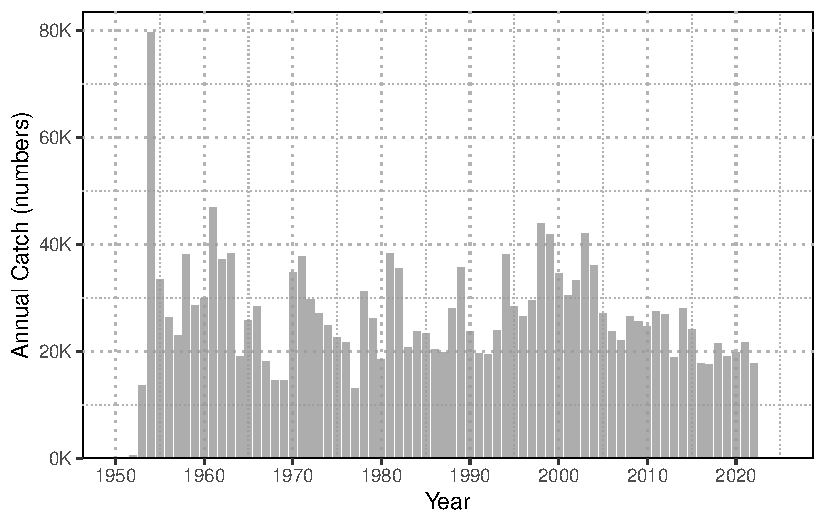
\includegraphics[keepaspectratio]{swpo-mls-bayesian-assessments_files/figure-pdf/fig-annual-catch-1.pdf}}

}

\caption{\label{fig-annual-catch}Annual catch of Southwest Pacific Ocean
striped marlin (1952-2022). Catch data shows initial low removals in
early years, a peak in 1954, followed by relatively stable catches with
a slight decline in recent decades.}

\end{figure}%

\newpage

\begin{figure}[H]

\centering{

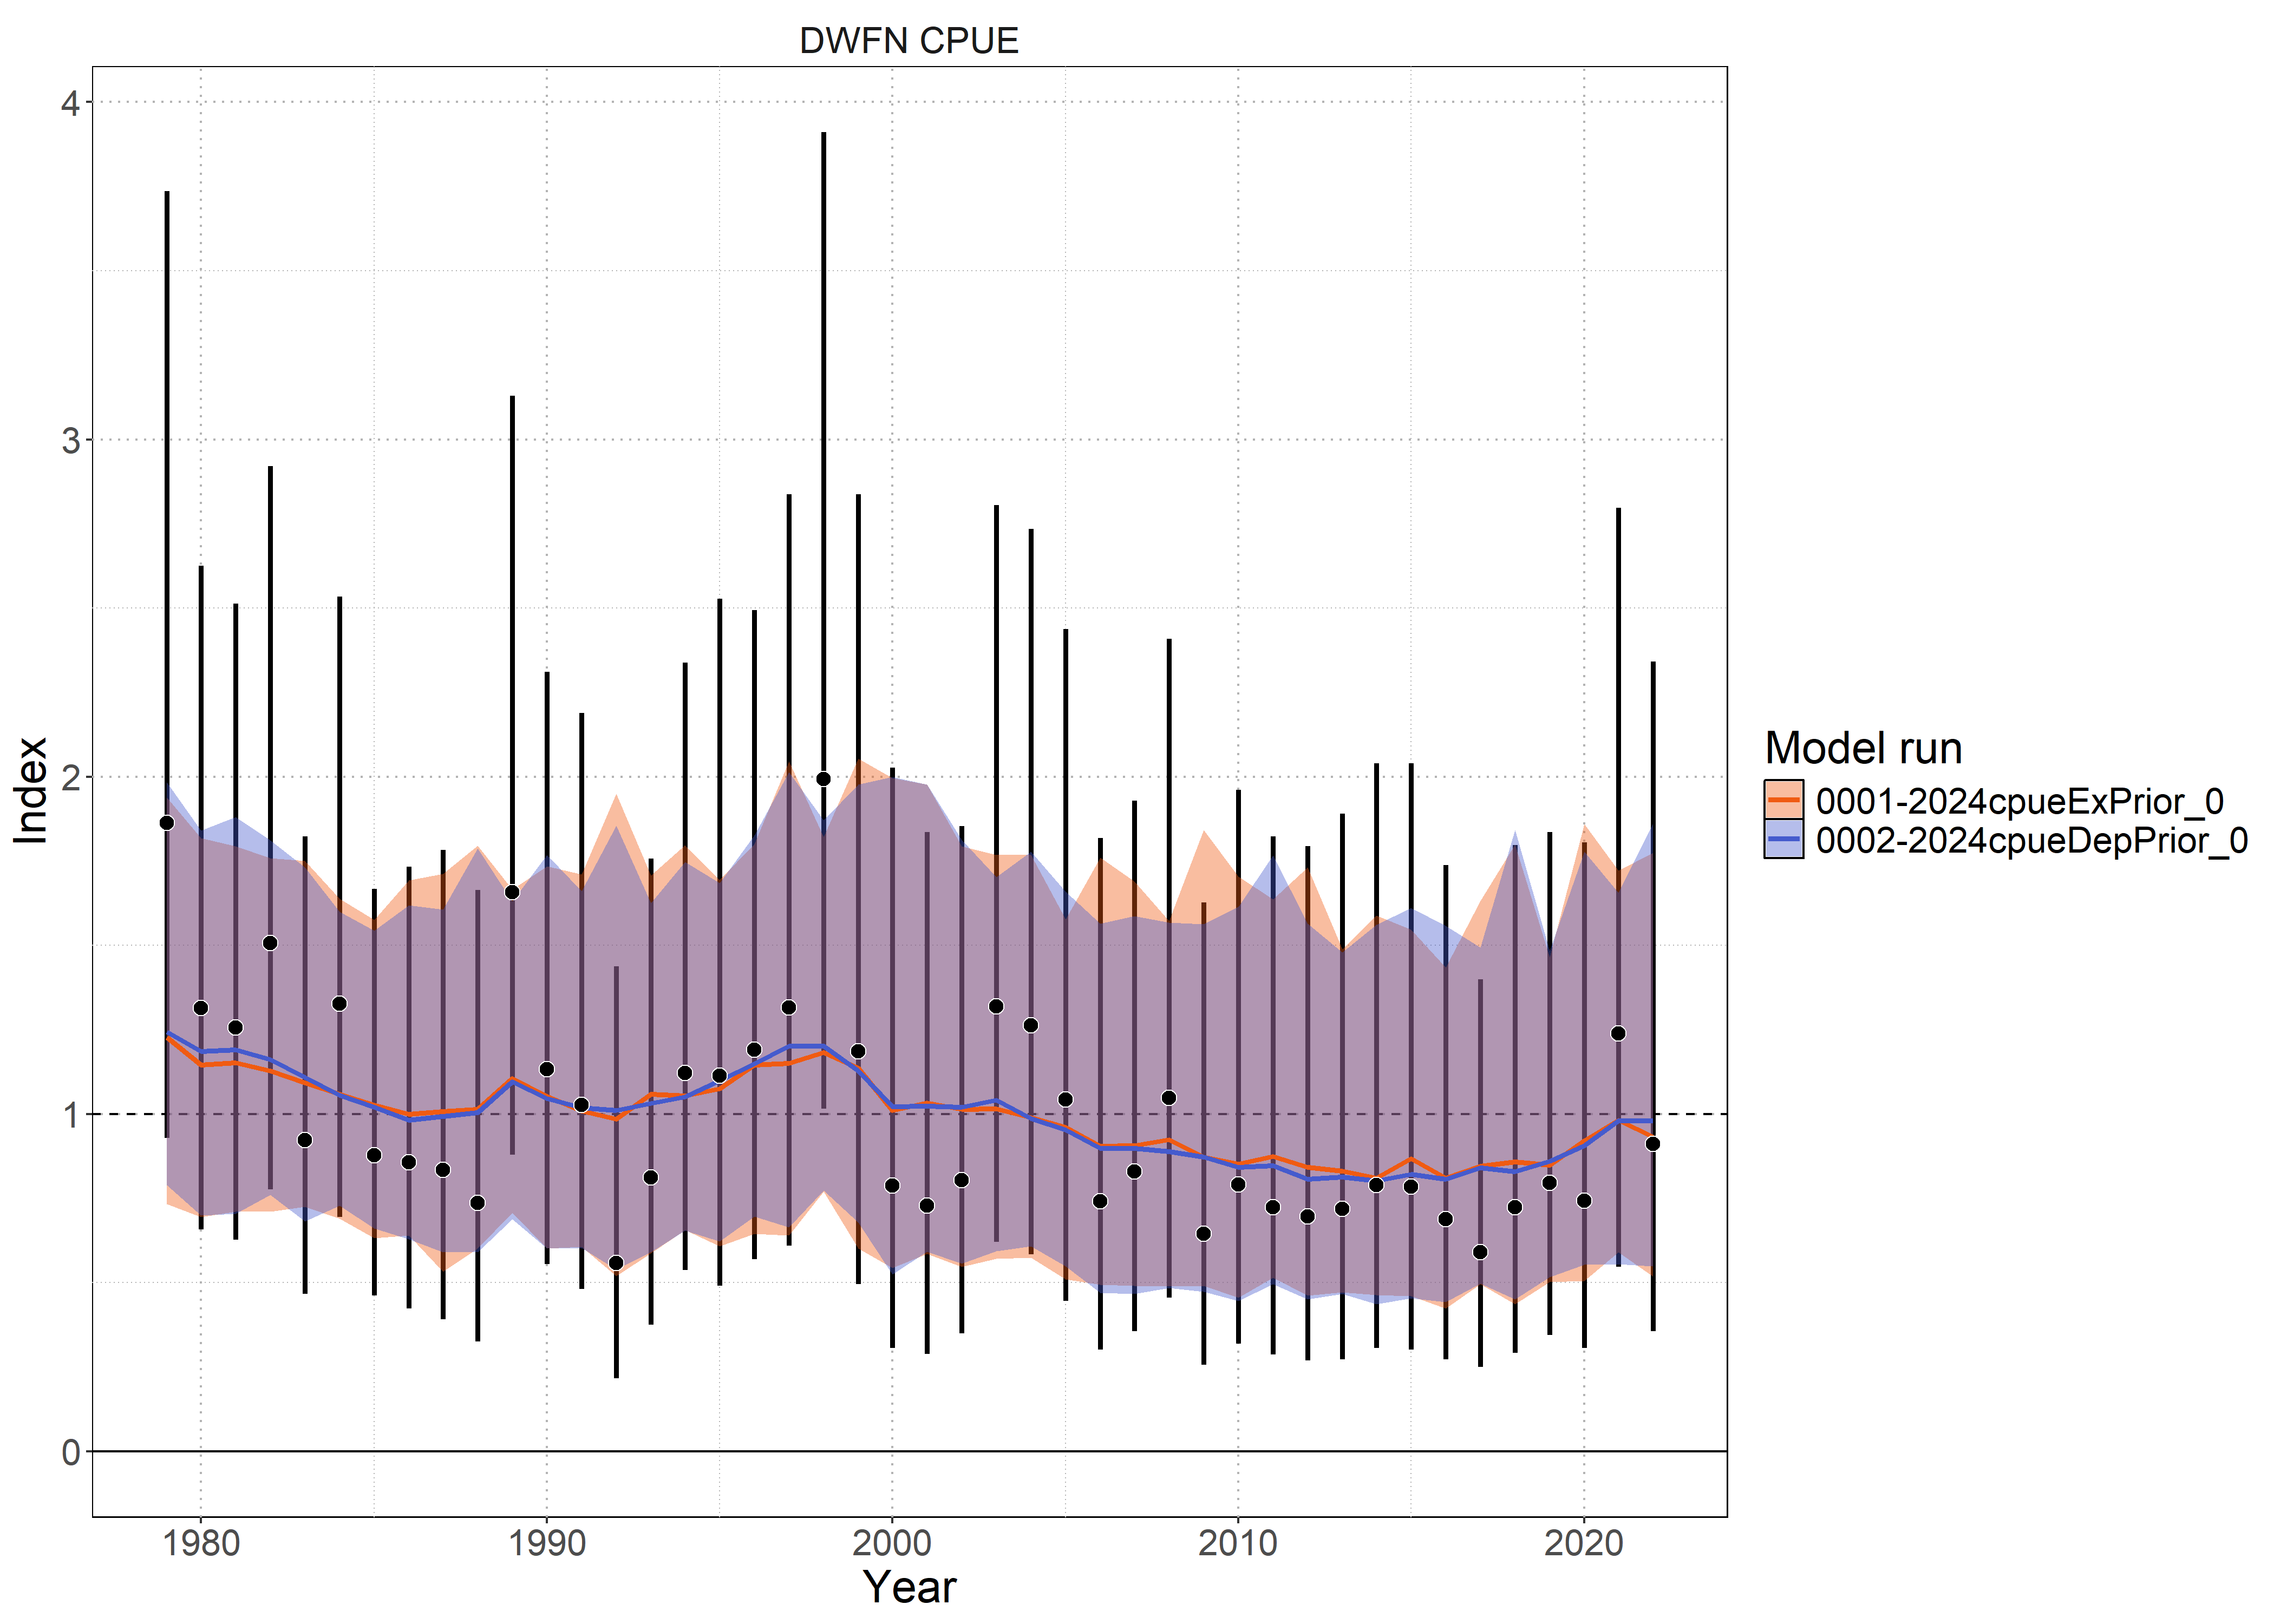
\includegraphics[width=1\linewidth,height=\textheight,keepaspectratio]{../plots/model_comparison/comparisons/comparison_index_fit_ppd.png}

}

\caption{\label{fig-idx-fit}Standardized index (black points),
observation error (black bars), and posterior predicted model fits
(colored lines) with associated 95\% credible interval (colored
shading).}

\end{figure}%

\newpage

\begin{figure}[H]

\centering{

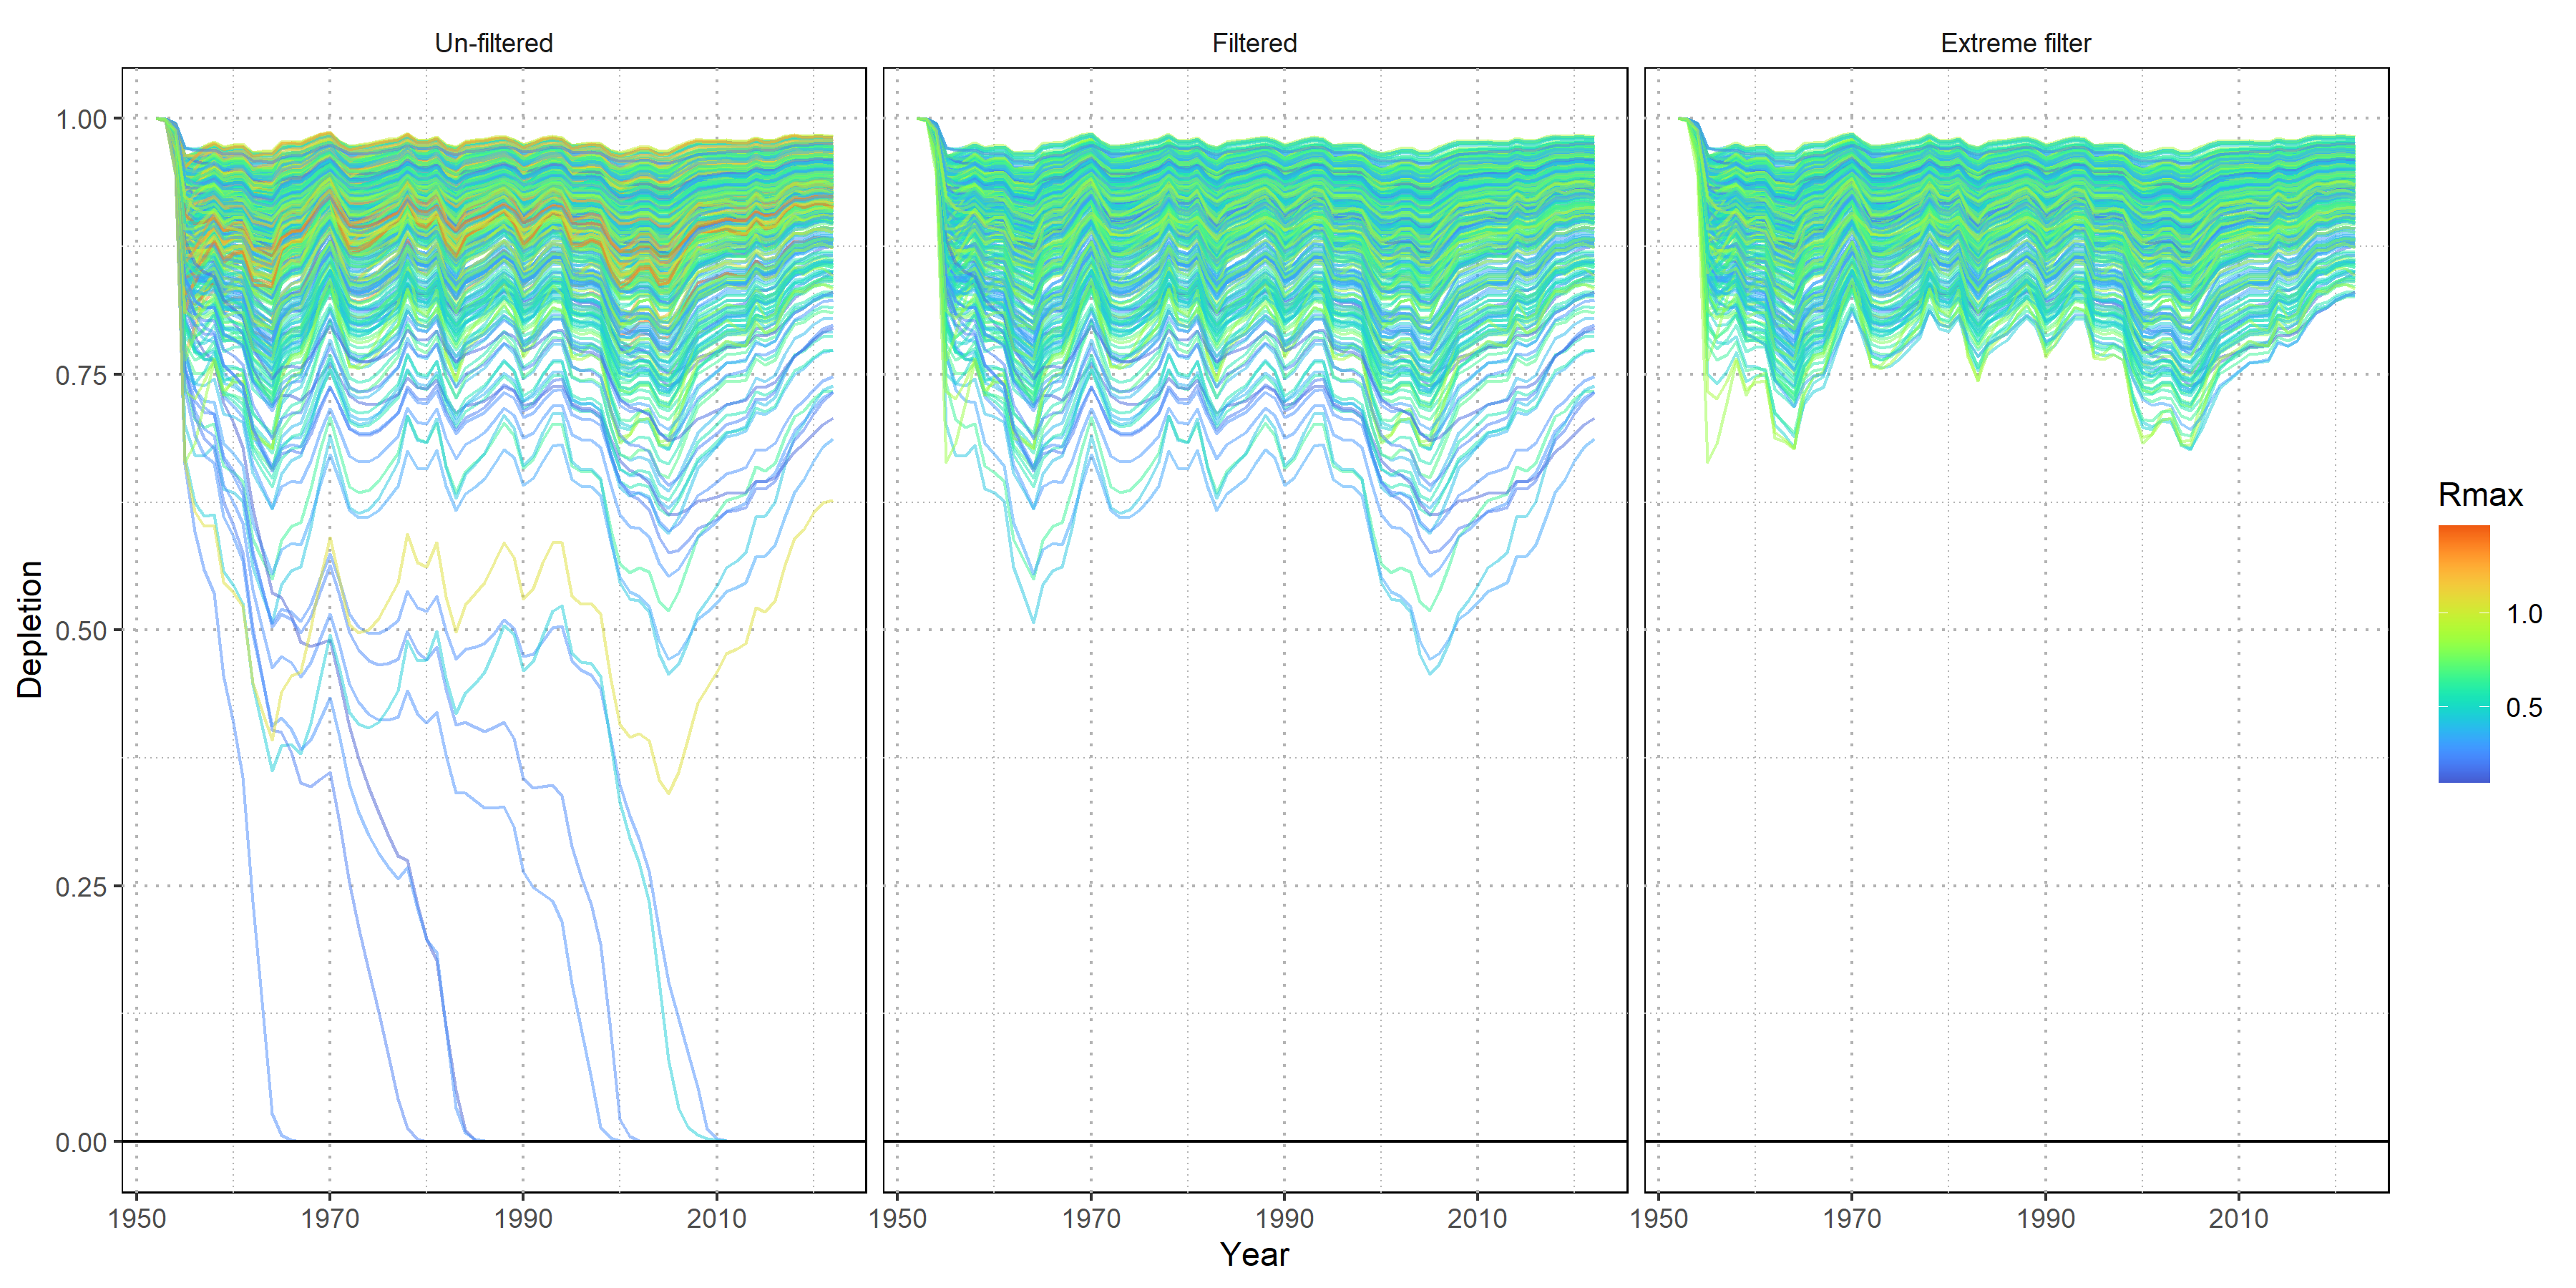
\includegraphics[width=1\linewidth,height=\textheight,keepaspectratio]{../plots/pushforward/prior_push.sim_dep.png}

}

\caption{\label{fig-pushforward}Prior pushforward check for population
depletion trajectories under different biological parameter filtering
scenarios. Each line represents a simulated population trajectory
colored by maximum intrinsic rate of increase (\(R_{max}\)). Left panel
shows unfiltered \(R_{max}\), middle panel shows filtered \(R_{max}\),
and right panel shows extreme filtering.}

\end{figure}%

\newpage

\begin{figure}[H]

\centering{

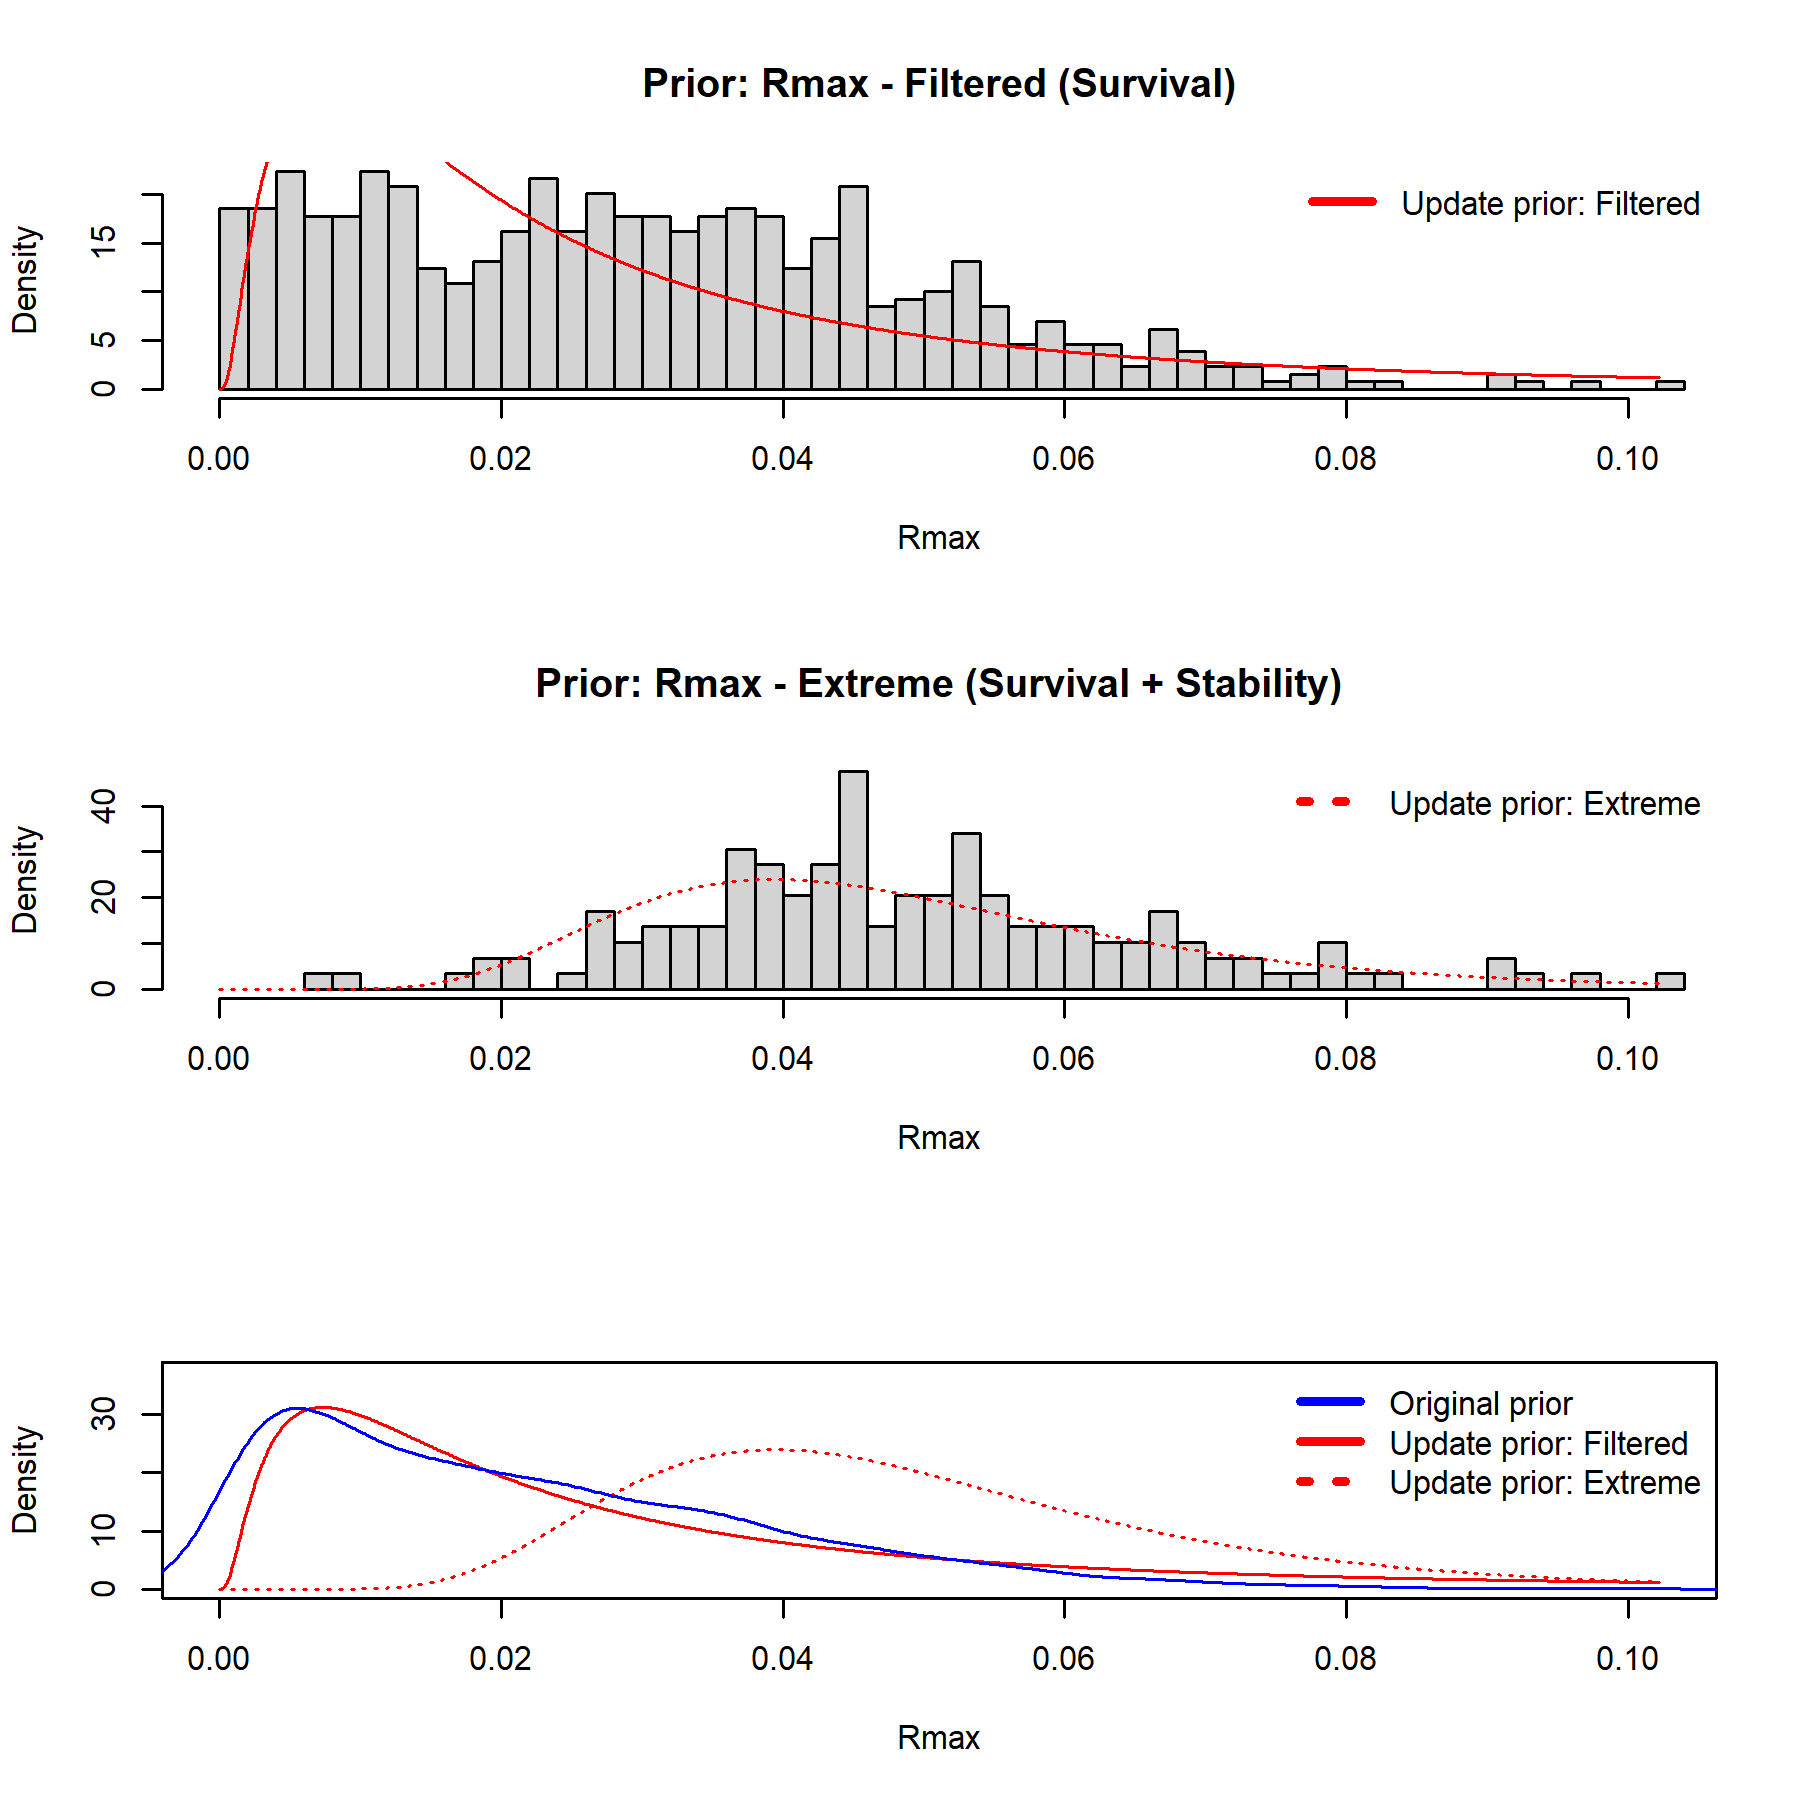
\includegraphics[width=1\linewidth,height=\textheight,keepaspectratio]{../plots/pushforward/prior.rmax.png}

}

\caption{\label{fig-rmax-prior}Prior distributions for maximum intrinsic
rate of population increase \(R_{max}\). Upper panel: Gray histogram is
the \(R_{max}\) values from the numerical simulation which meet baseline
filtering levels. Red line is fitted lognormal distribution. Middle
panel: Gray histogram is the \(R_{max}\) values from the numerical
simulation which meet extreme filtering levels. Dotted red line is
fitted lognormal distribution. Bottom panel: Original distribution of
\(R_{max}\) values from numerical simulation (gray), those from viable
populations (blue), and the two lognormal priors (red).}

\end{figure}%

\newpage

\begin{figure}[H]

\centering{

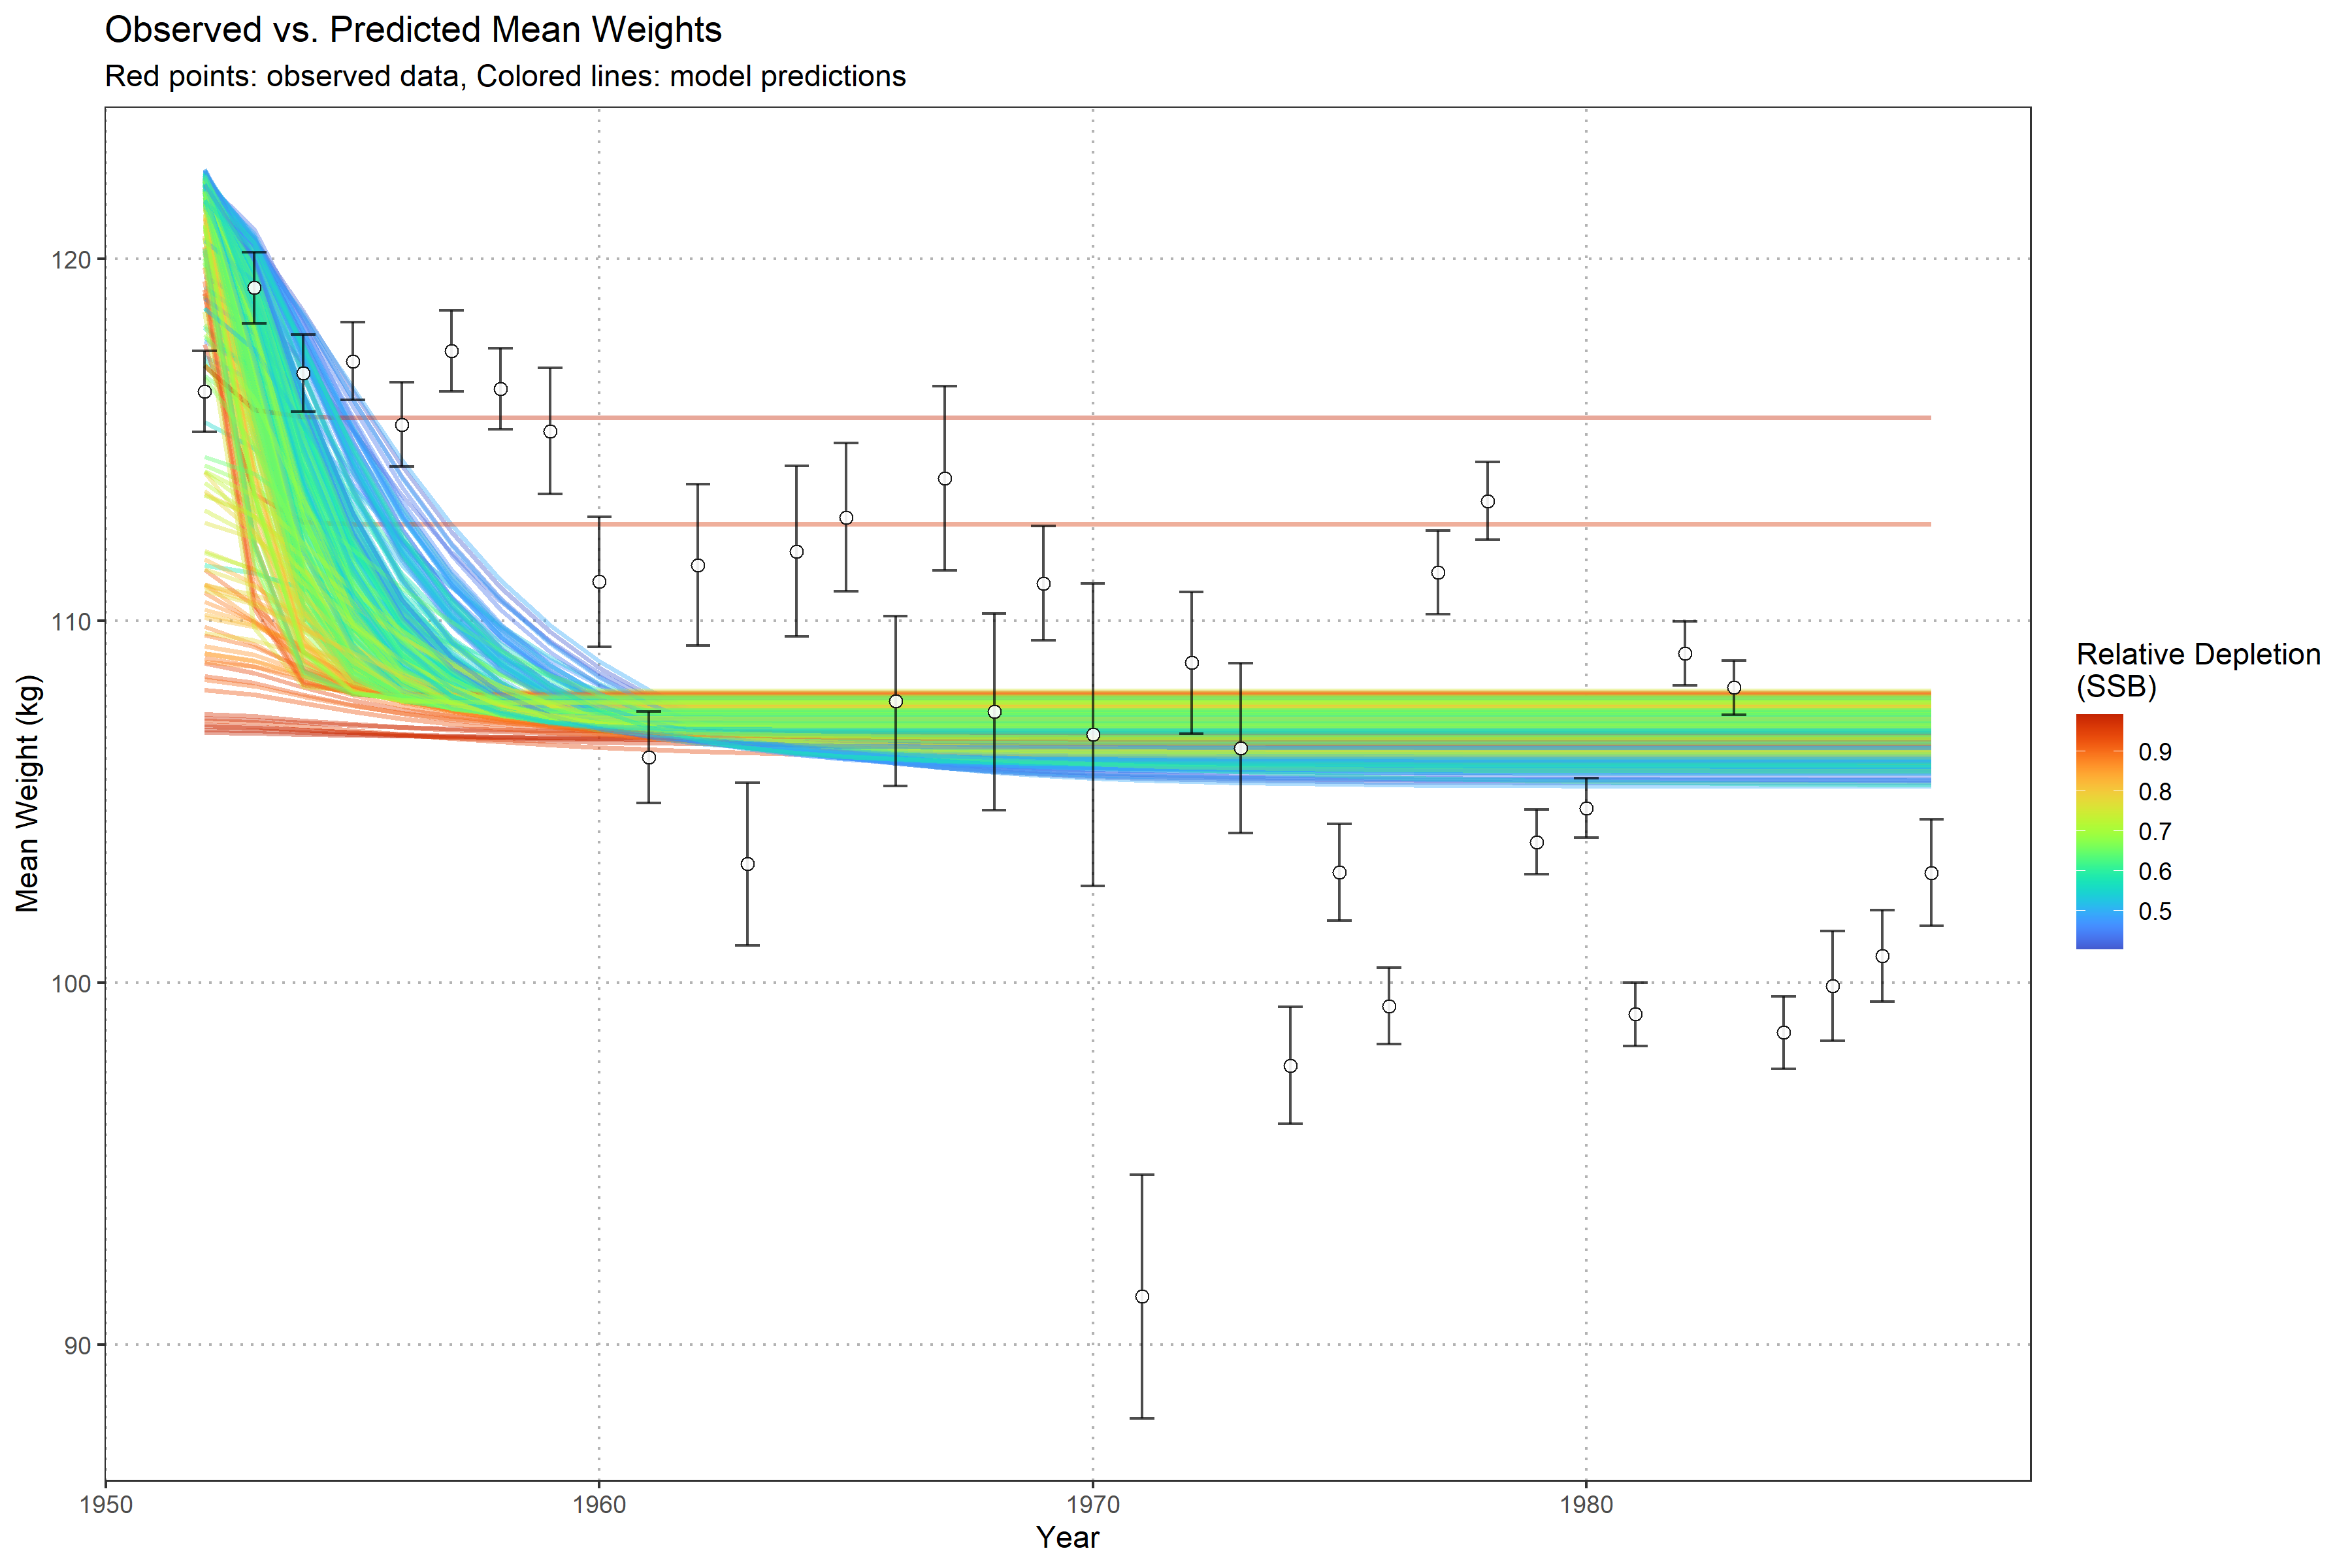
\includegraphics[width=1\linewidth,height=\textheight,keepaspectratio]{../plots/depletion/mean_weight_comparison.png}

}

\caption{\label{fig-gedamke}Observed versus predicted mean weights from
New Zealand recreational fishery data. Points show observed mean weights
with error bars, colored lines show model predictions from the
transitional mean weight model colored by relative spawning stock
biomass (SSB) depletion.}

\end{figure}%

\newpage

\begin{figure}[H]

\centering{

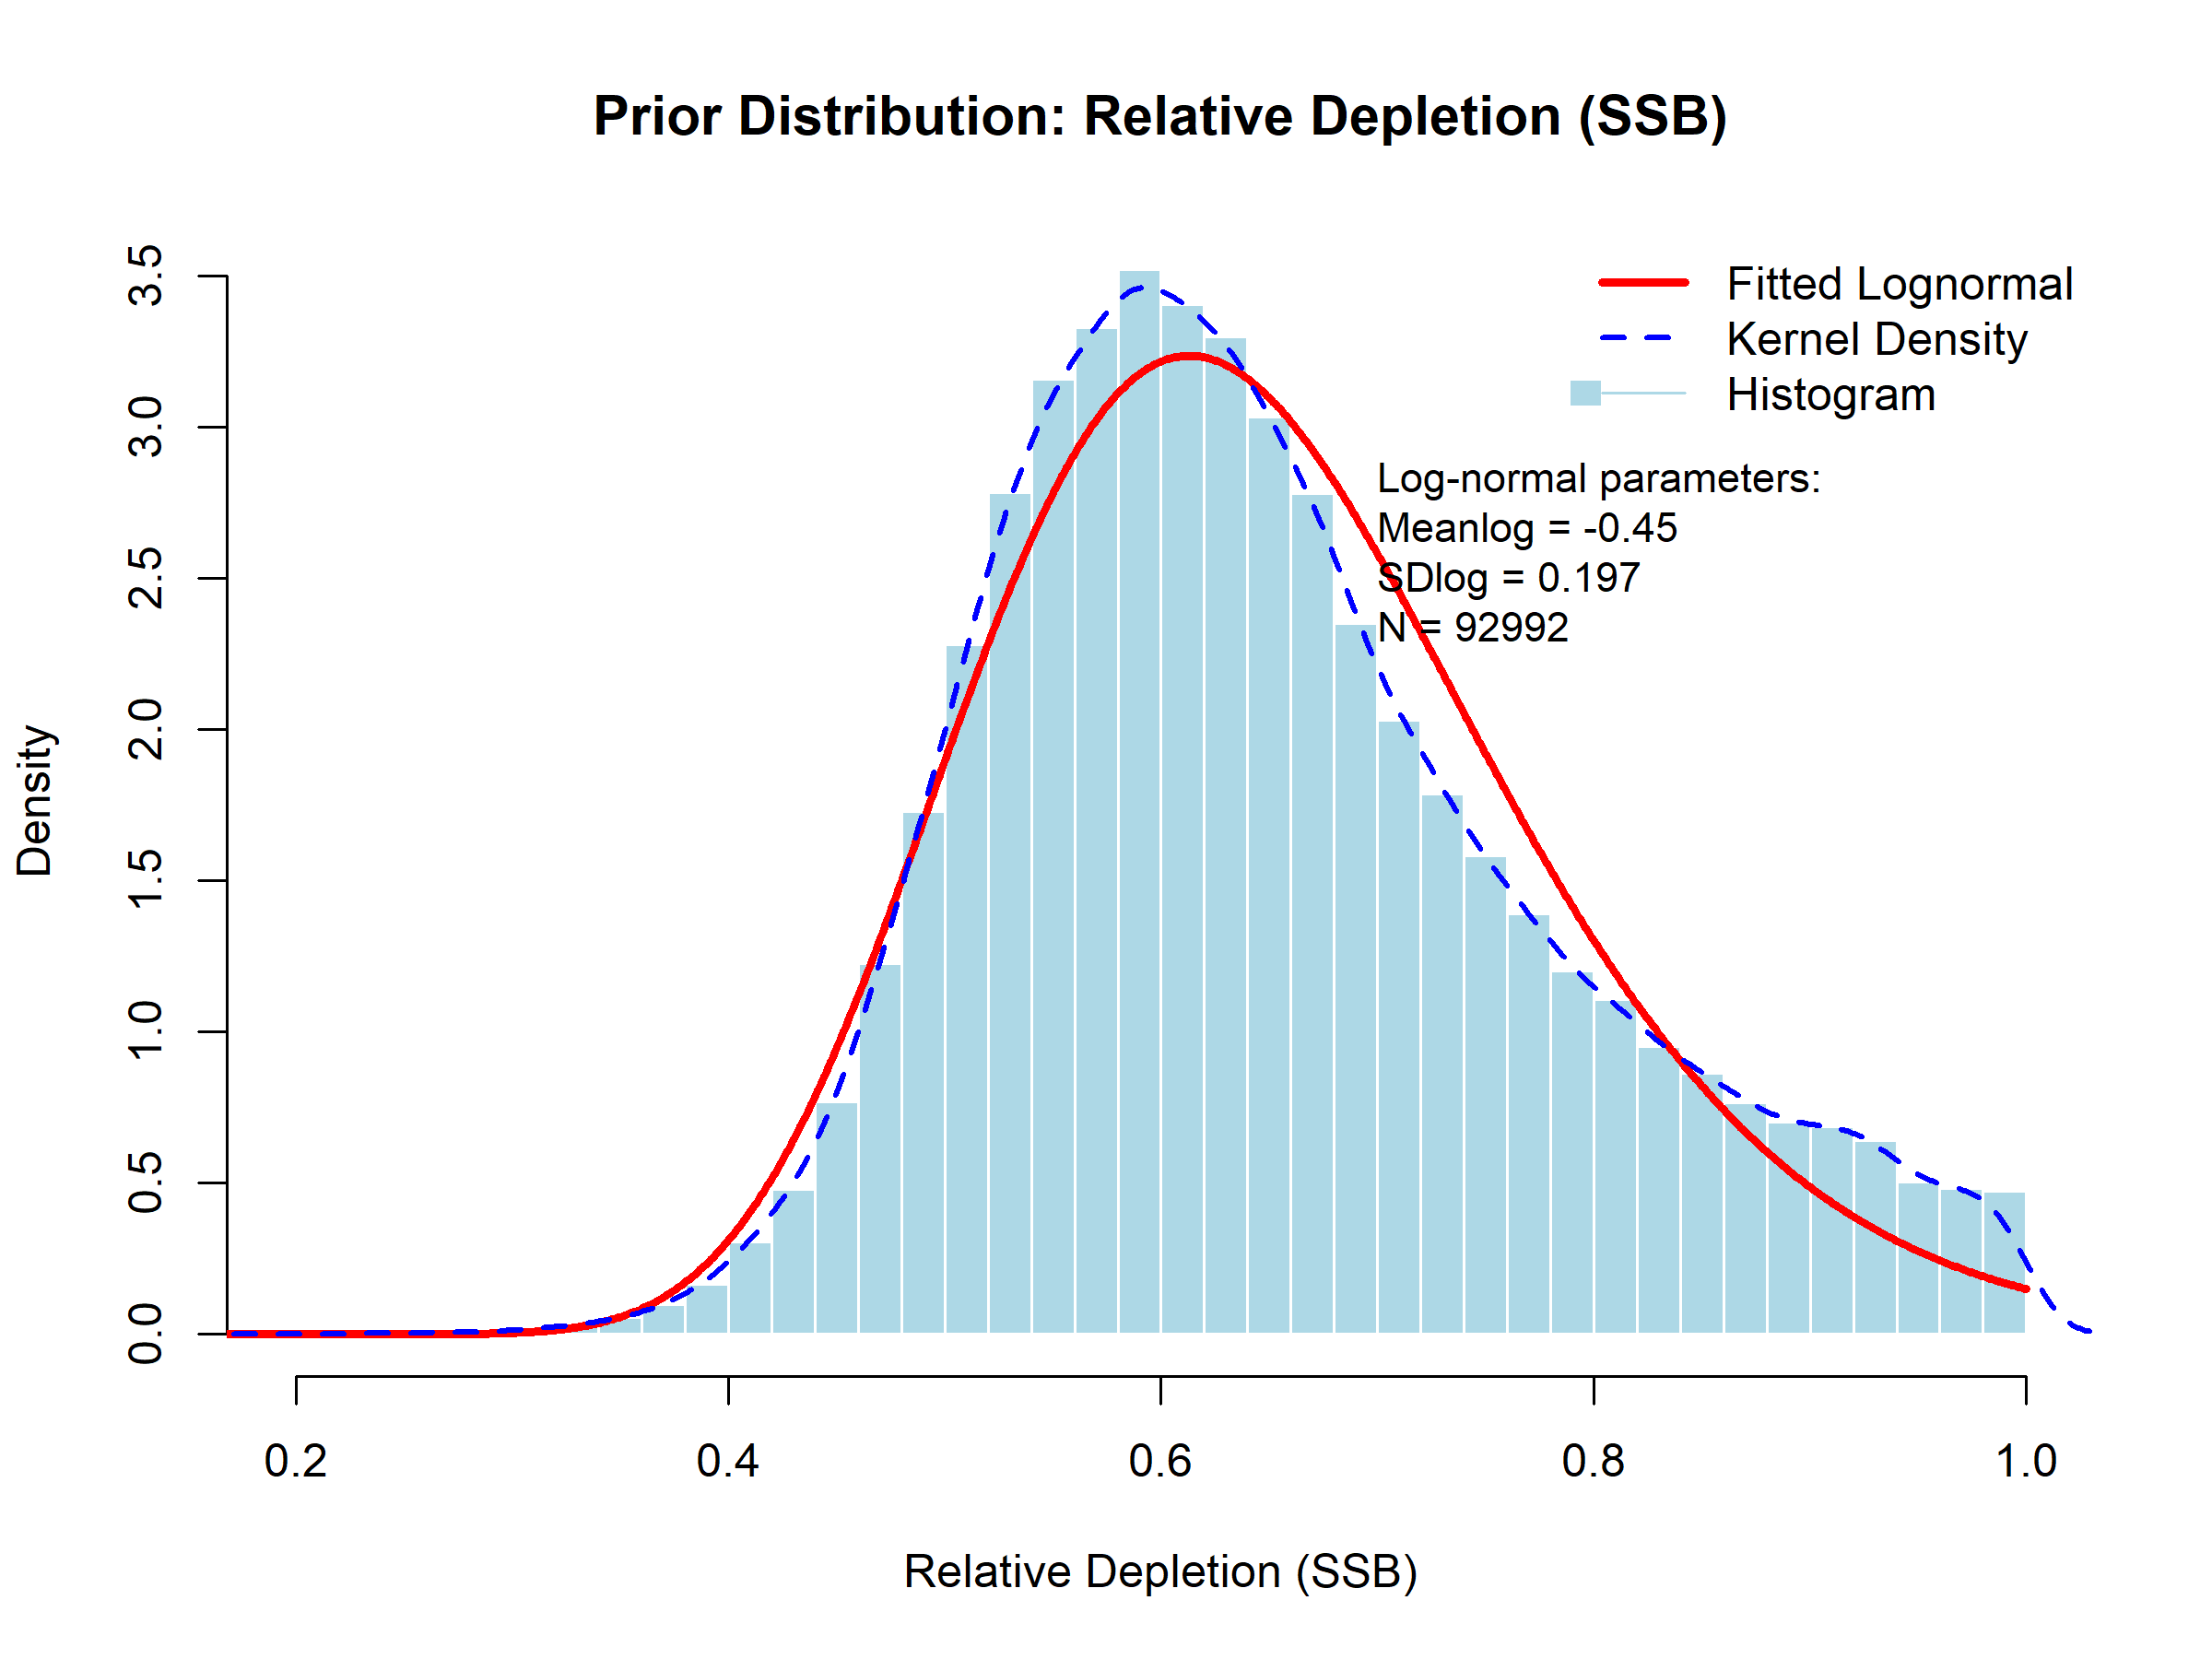
\includegraphics[width=1\linewidth,height=\textheight,keepaspectratio]{../plots/depletion/prior_rel_dep_ssb.png}

}

\caption{\label{fig-dep-prior}Prior distribution for relative depletion
in 1988 derived from New Zealand recreational weight data. Light blue
histogram shows depletion estimates from biological parameter
combinations that successfully fit the transitional mean weight model.
Blue dashed line shows kernel density estimate, red line shows fitted
lognormal distribution used as prior in the depletion-constrained BSPM.}

\end{figure}%

\newpage

\begin{figure}[H]

\centering{

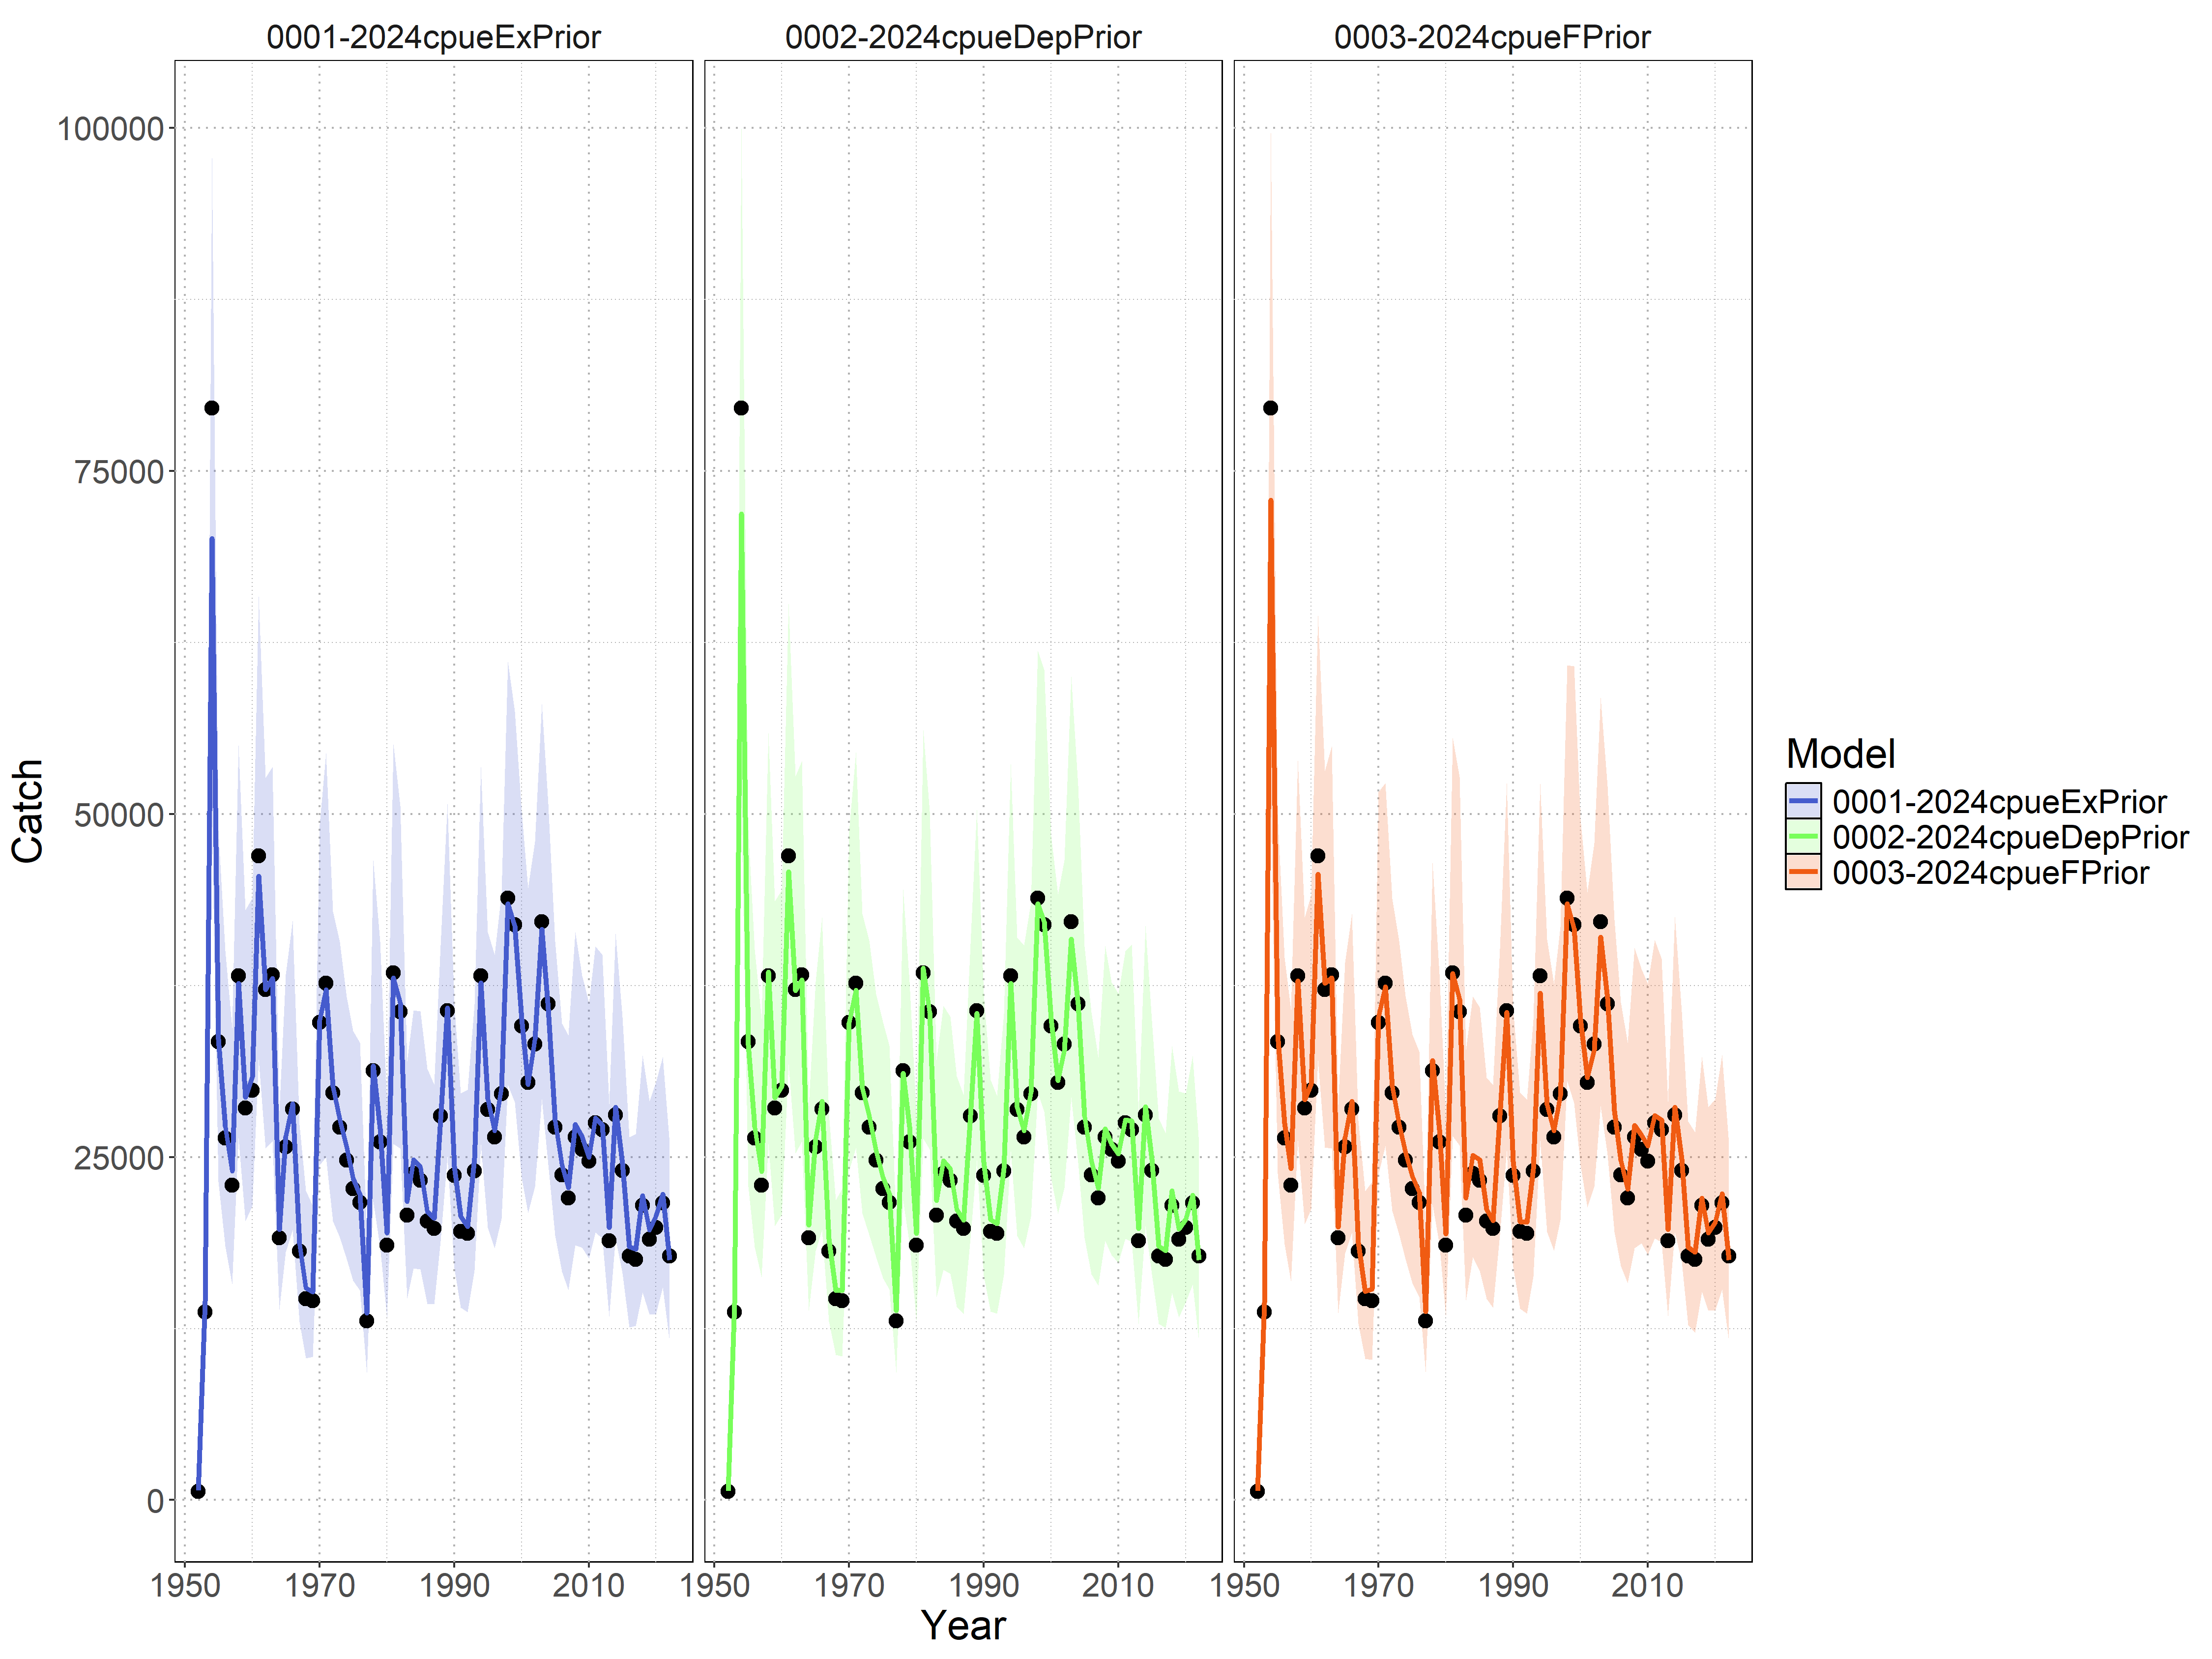
\includegraphics[width=1\linewidth,height=\textheight,keepaspectratio]{../plots/predicted_catch.png}

}

\caption{\label{fig-pred-catch}Time series of observed catch (black dots
with uncertainty bounds) and model-predicted catch for two Bayesian
surplus production models fitted to SWPO striped marlin data from
1950-2022. The left panel shows model \inlinecode{0001-2024cpueExPrior}
(baseline model with expert priors) and the right panel shows model
\inlinecode{0002-2024cpueDepPrior} (depletion-constrained model
incorporating 1988 depletion prior from New Zealand recreational weight
data). Colored lines represent posterior median predictions with shaded
uncertainty bands showing 95\% credible intervals.}

\end{figure}%

\newpage

\begin{figure}[H]

\centering{

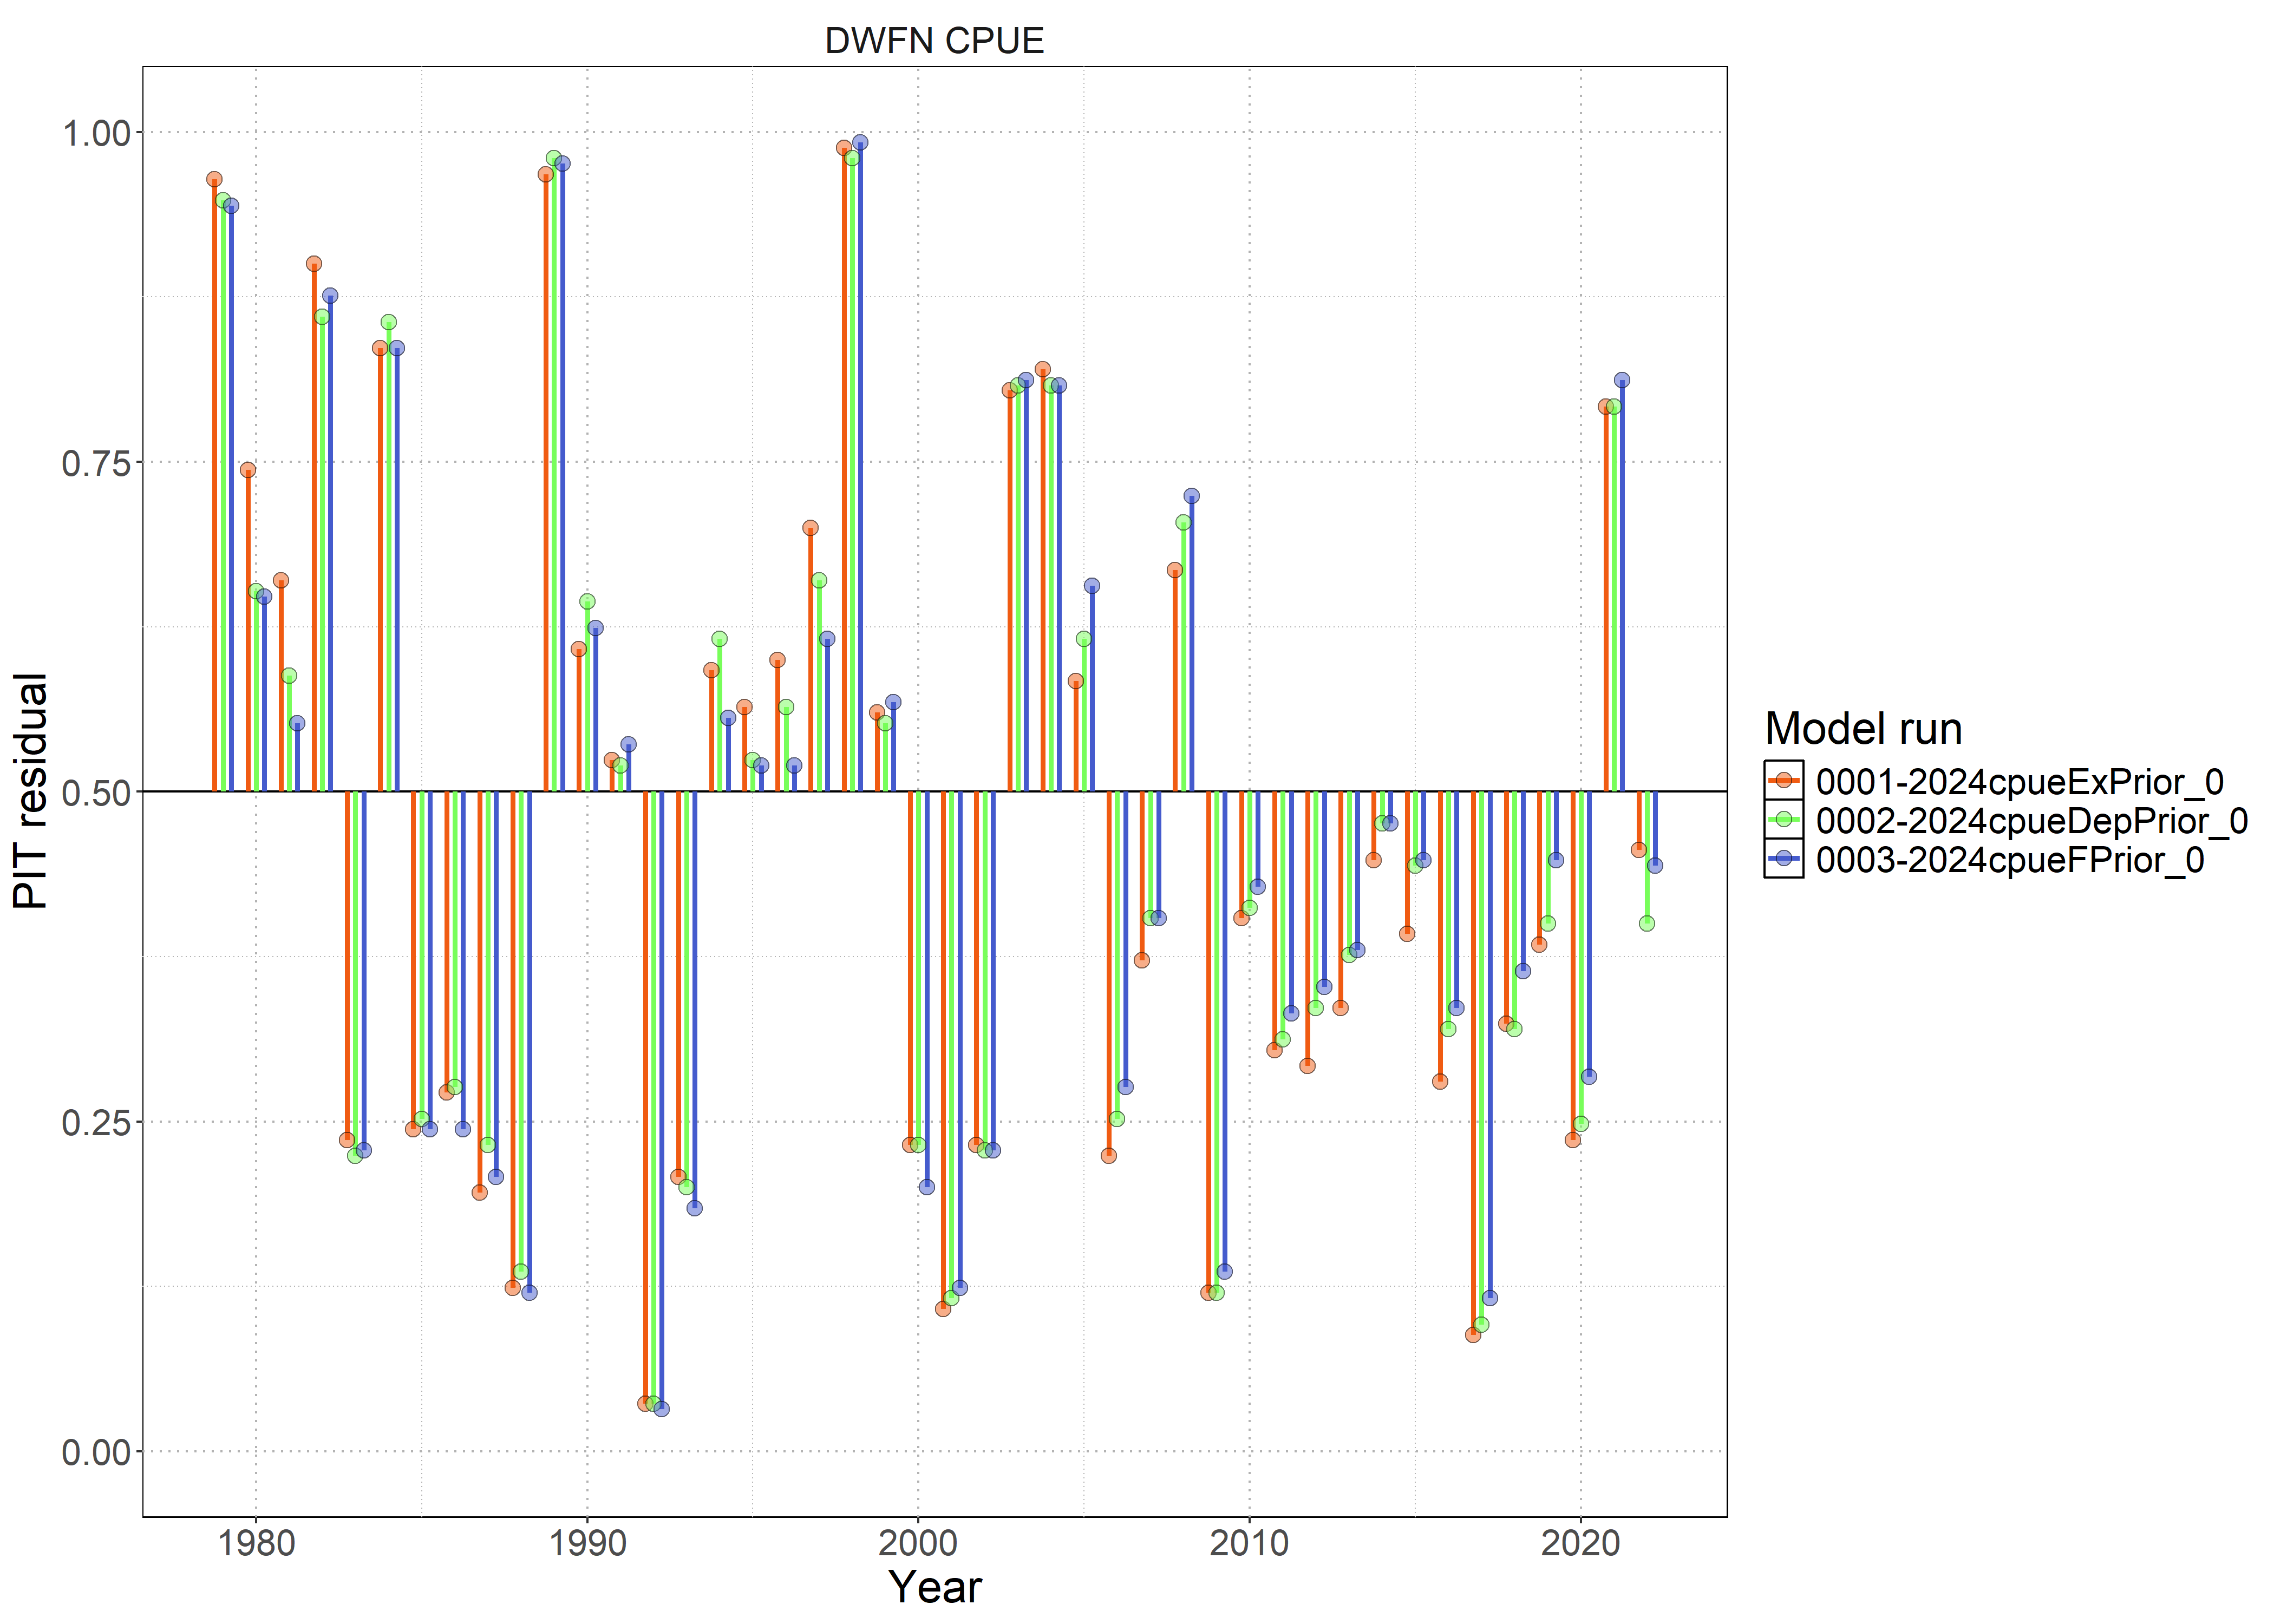
\includegraphics[width=1\linewidth,height=\textheight,keepaspectratio]{../plots/model_comparison/comparisons/comparison_index_fit_residuals.png}

}

\caption{\label{fig-idx-residuals}Probability-integral transform (PIT)
style residuals from each model (colored points) fit to the standardized
index.}

\end{figure}%

\newpage

\begin{figure}[H]

\centering{

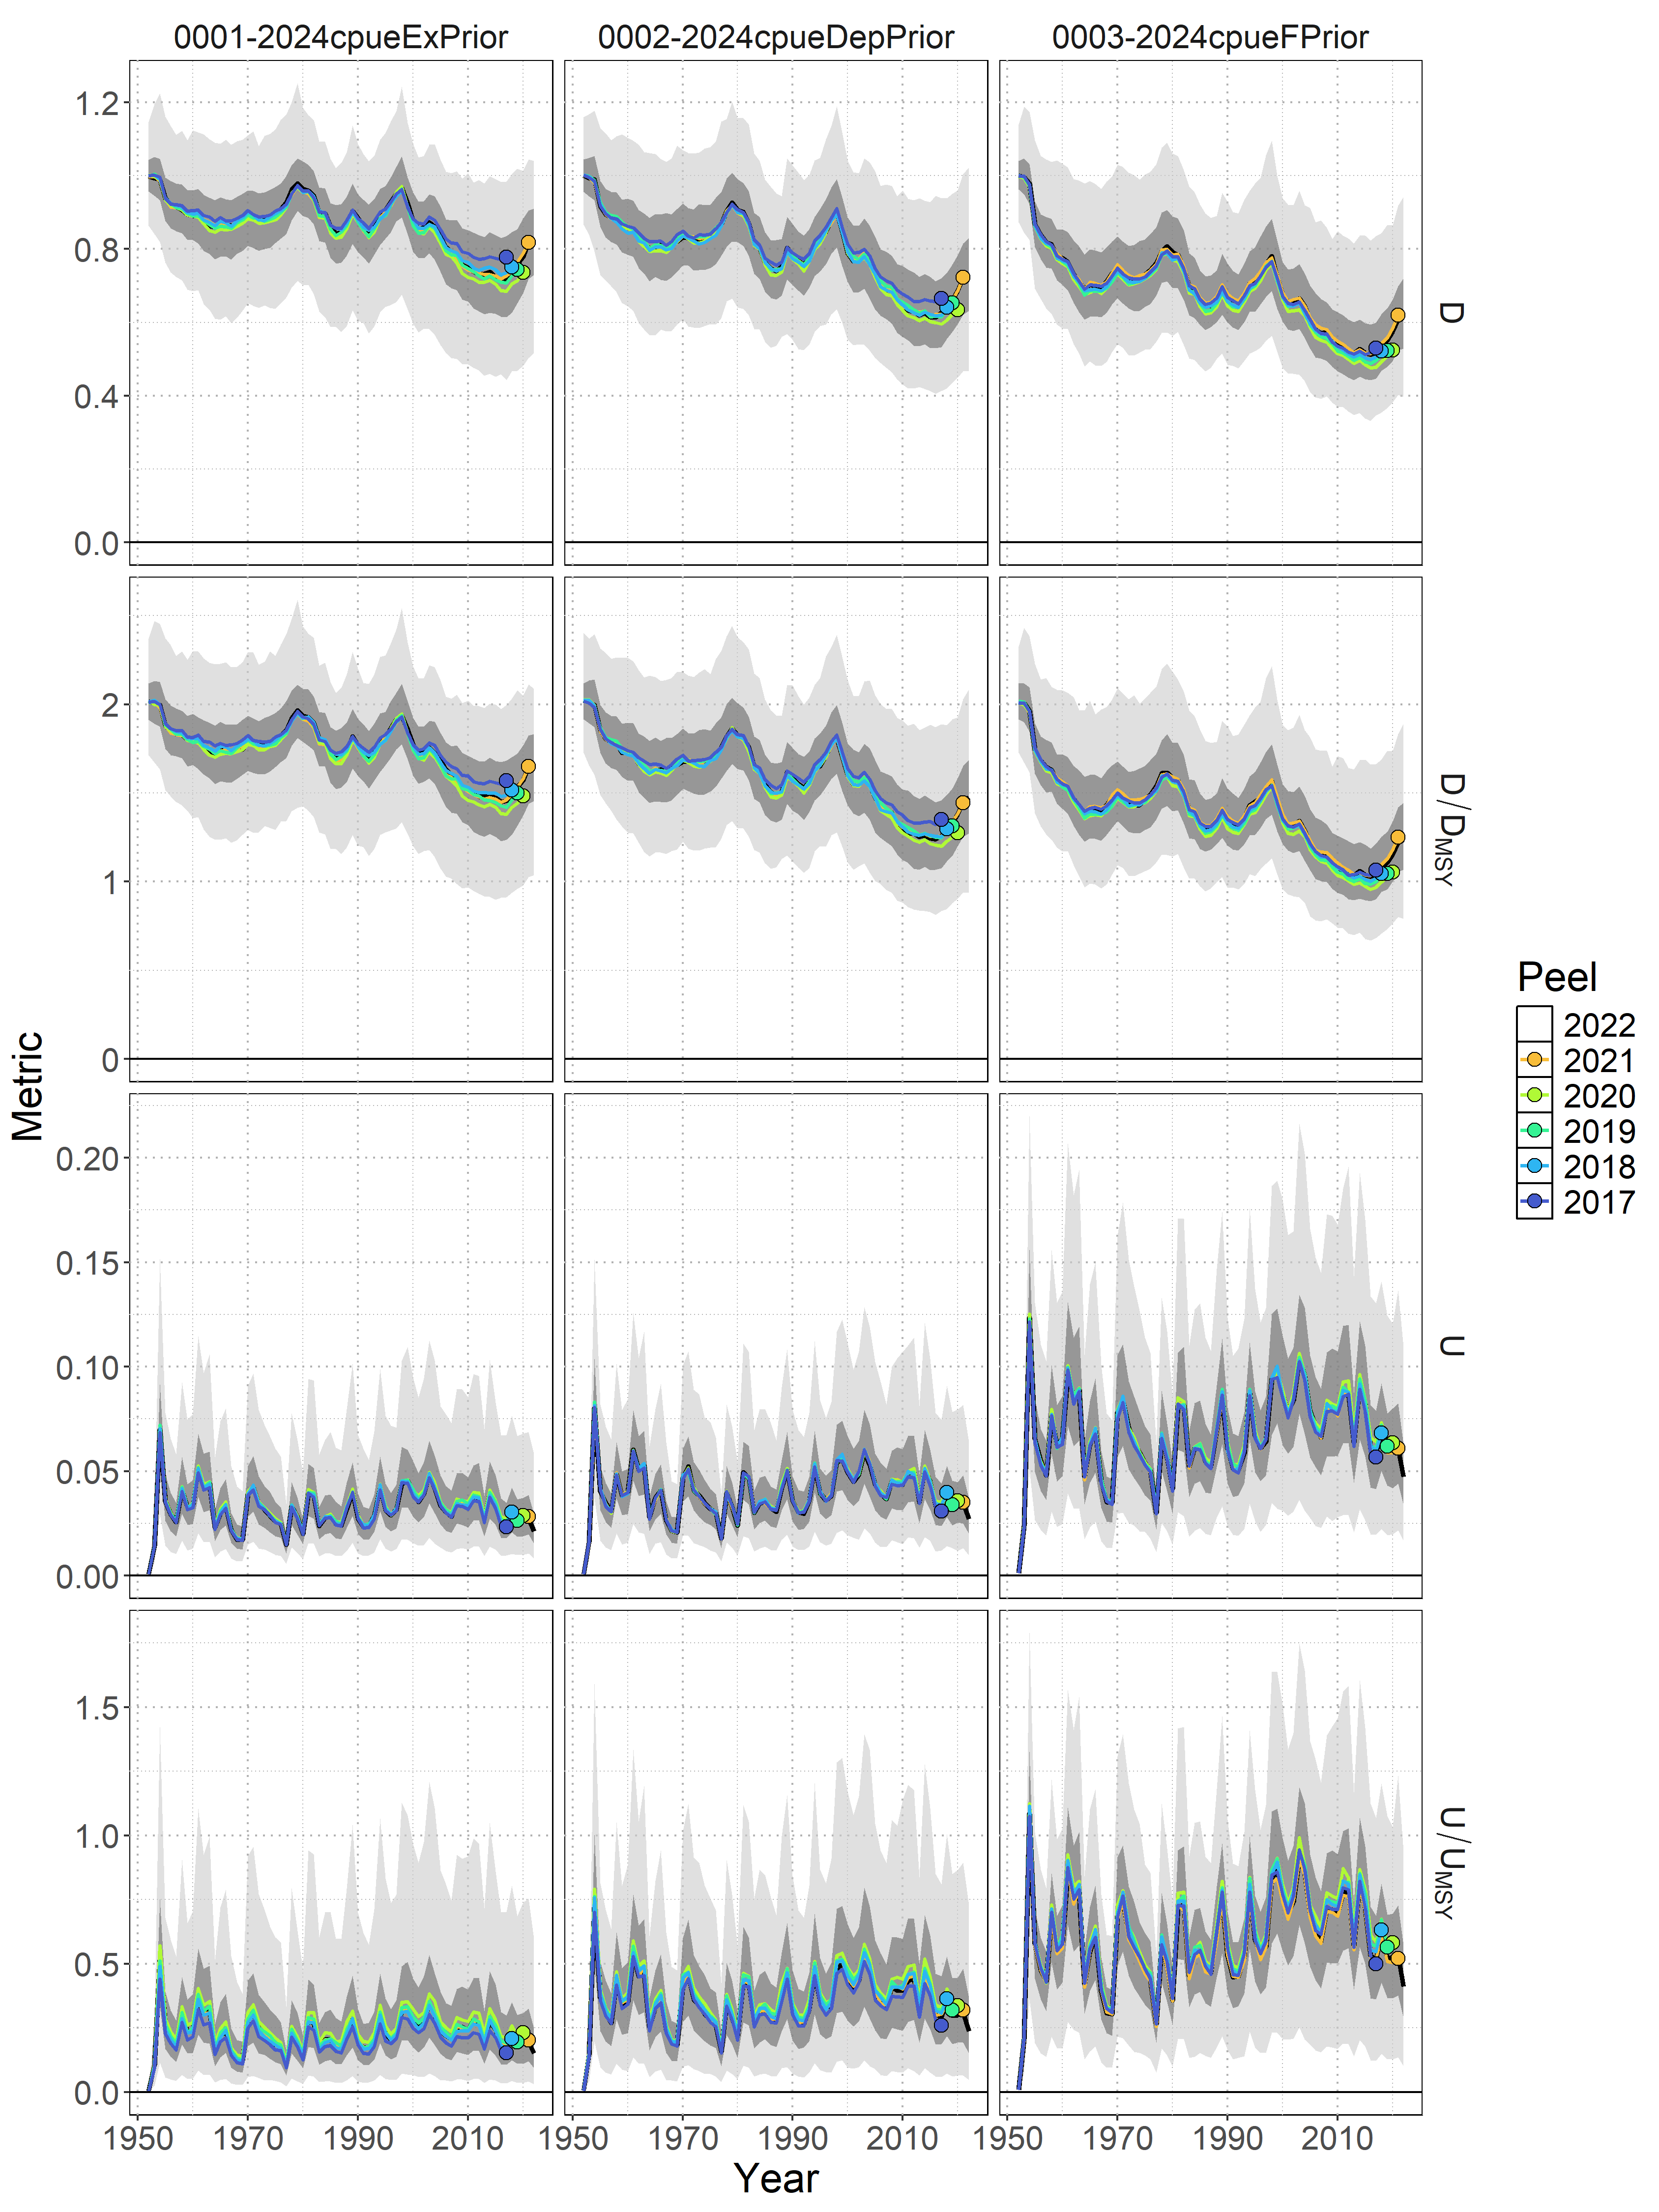
\includegraphics[width=0.9\linewidth,height=\textheight,keepaspectratio]{../plots/retro_analysis.png}

}

\caption{\label{fig-retro}Retrospective analysis for both models with
respect to time series of depletion \(D_t\), depletion relative to
depletion at MSY \(D_t/D_{MSY}\), exploitation rate \(U_t\), and
exploitation rate relative to the rate of exploitation that produces MSY
\(U_t/U_{MSY}\). The base model with data included through 2022 (black
line -- median; dark shading -- 50\% credible interval; light shading --
95\% credible interval) is shown relative to the retrospective models.
Colored lines correspond to the last year of index data and the colored
point indicates the estimate in the last year of the retrospective
peel.}

\end{figure}%

\newpage

\begin{figure}[H]

\centering{

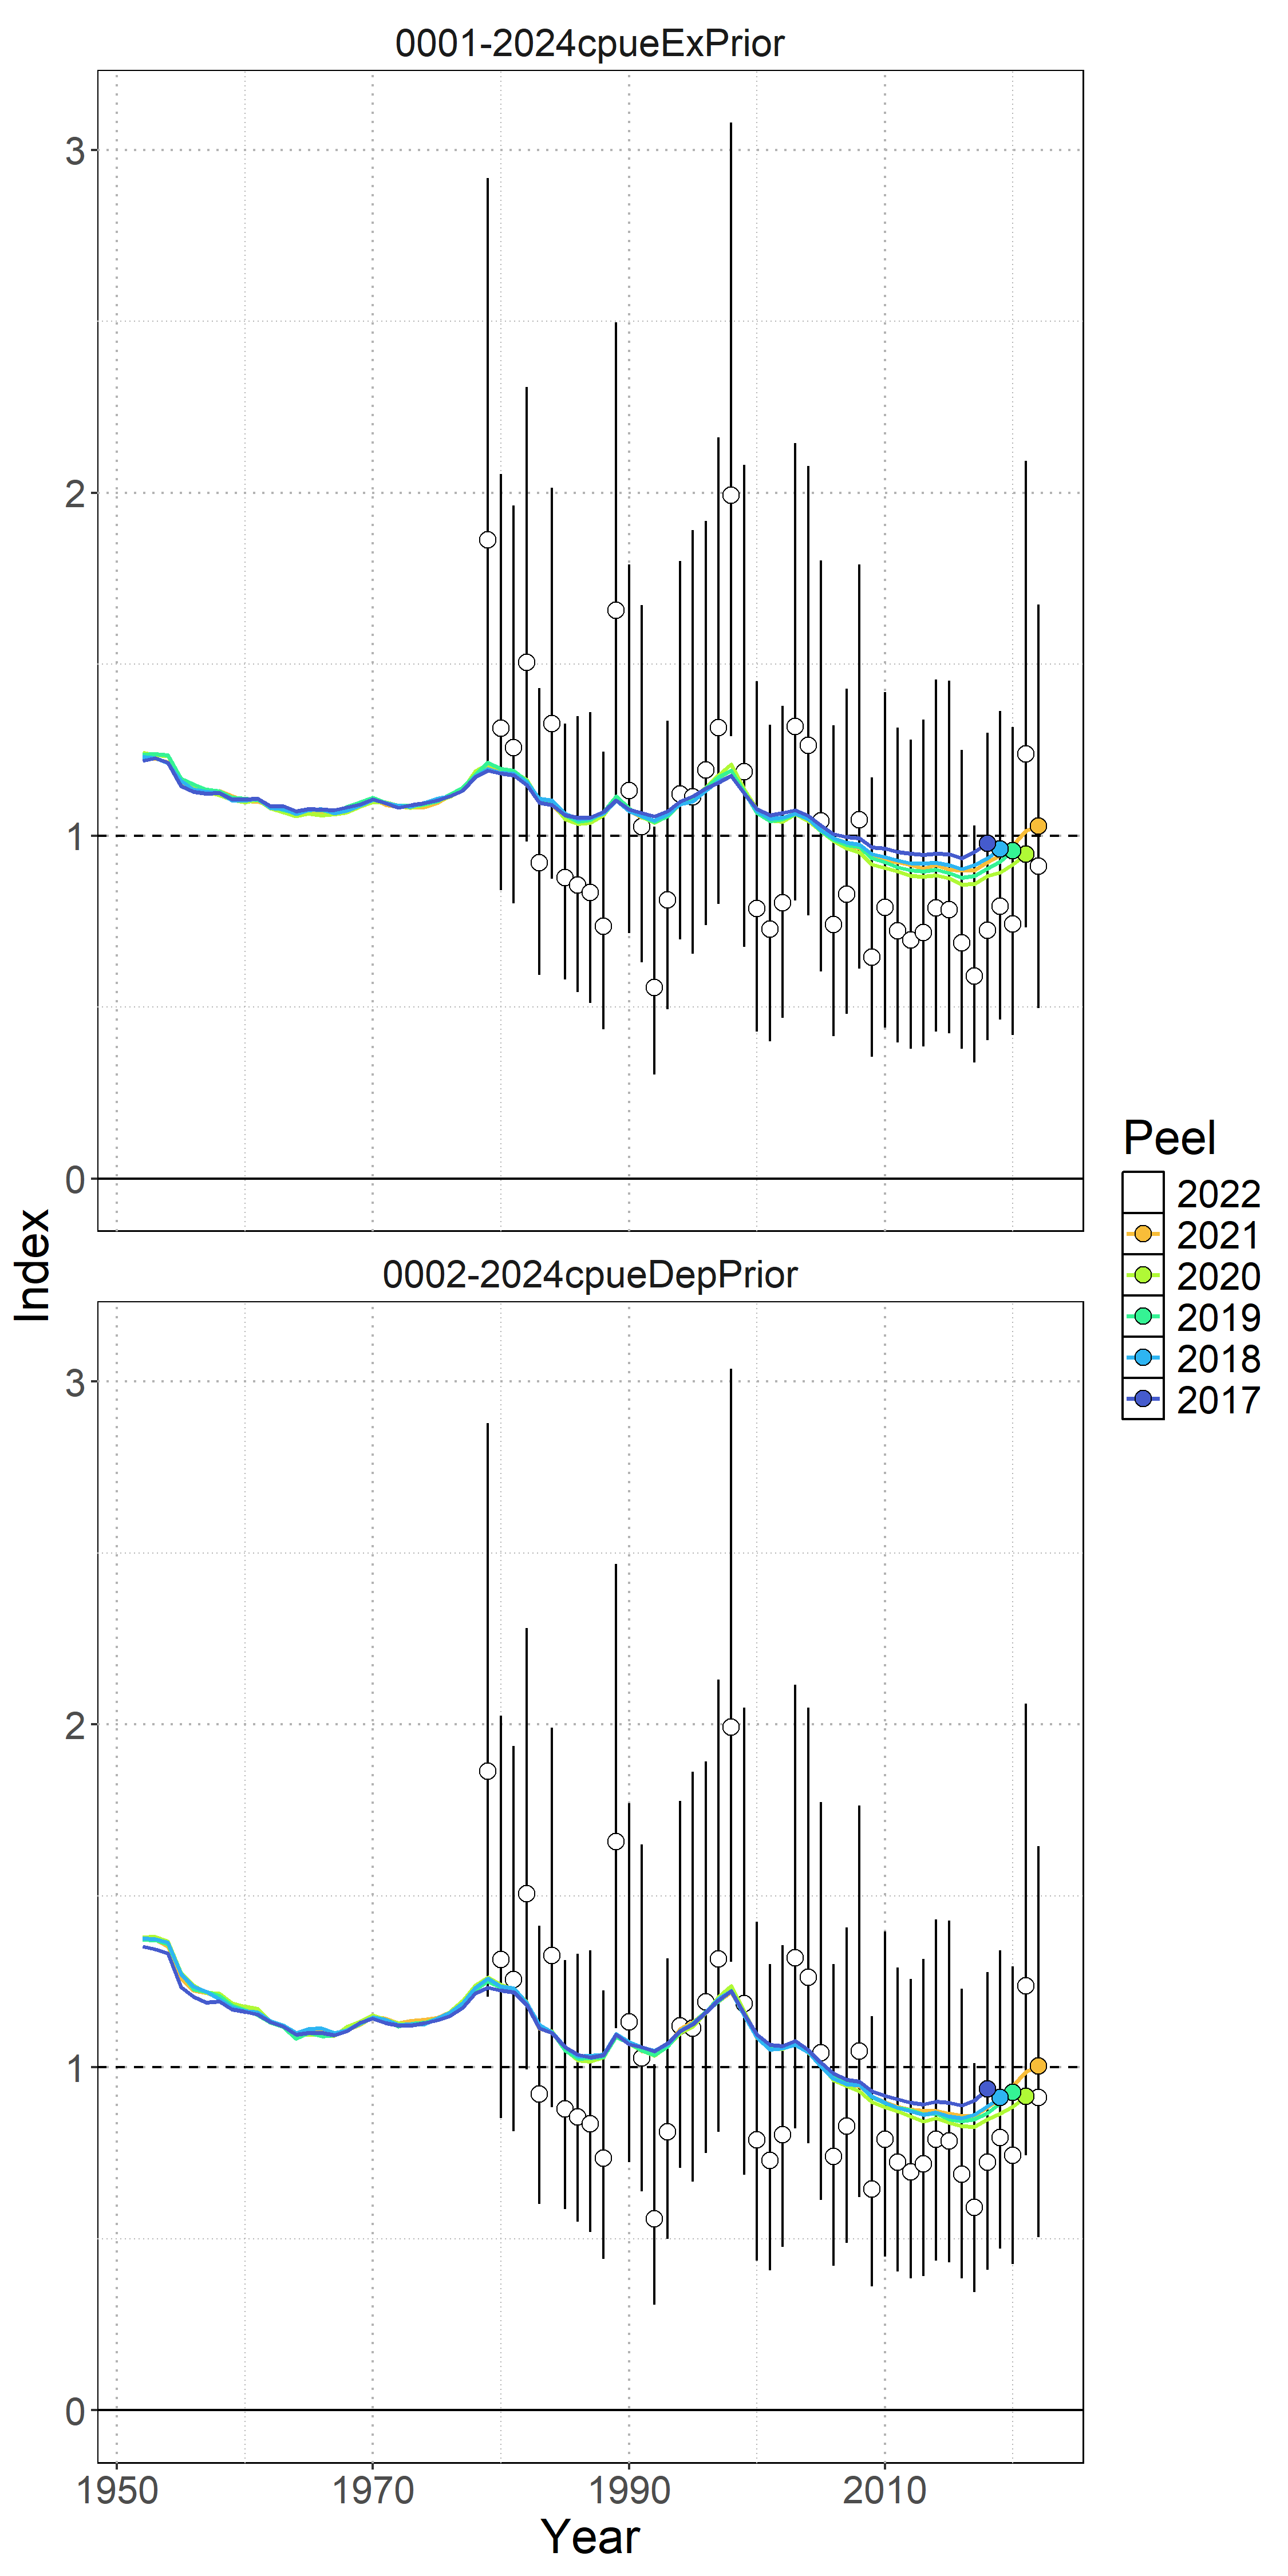
\includegraphics[width=\linewidth,height=0.9\textheight,keepaspectratio]{../plots/hcxval_analysis.png}

}

\caption{\label{fig-hcxval}Standardized indices of relative abundance
used in the Bayesian Surplus Production Model. Open circles show
observed values (standardized to mean of 1; black horizontal line) and
the vertical bars indicate the observation error (95\% confidence
interval). One year ahead `model-free' hindcast predictions are shown by
the colored lines, where the color indicates the last year of index data
seen by the model. The predicted value is shown one year-ahead with the
colored point.}

\end{figure}%

\newpage

\begin{figure}[H]

\centering{

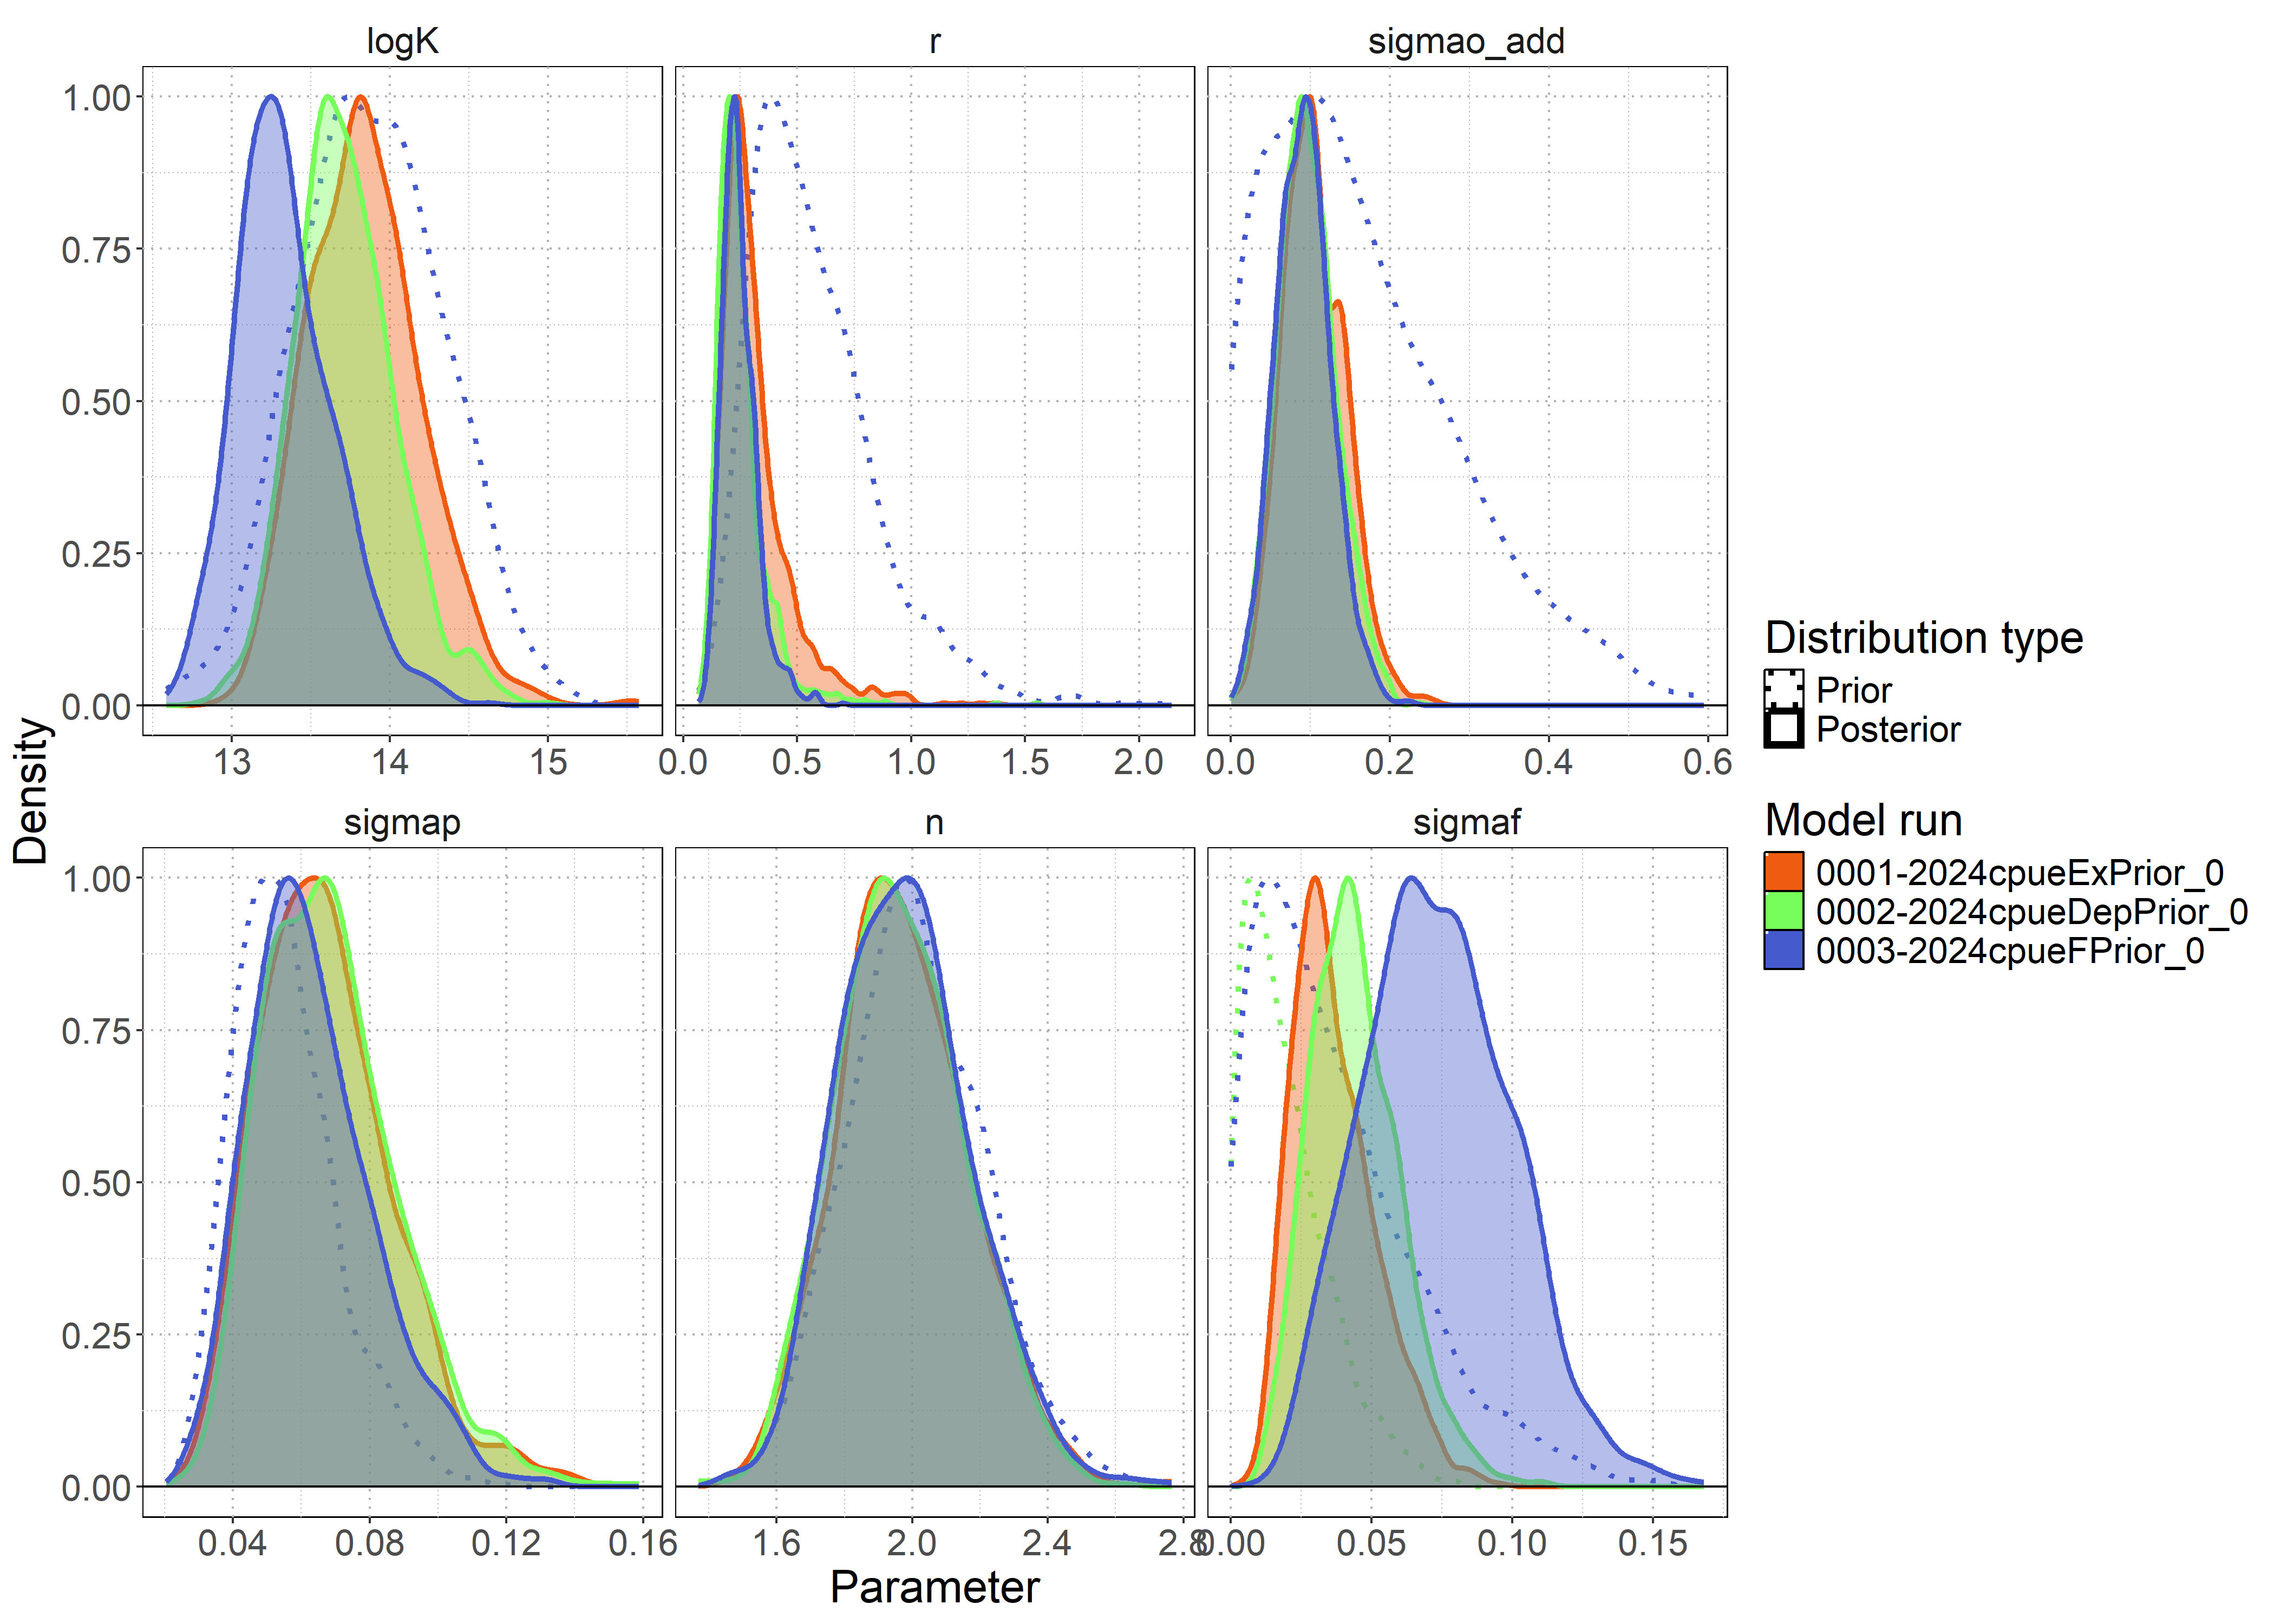
\includegraphics[width=1\linewidth,height=\textheight,keepaspectratio]{../plots/model_comparison/comparisons/comparison_prior_posterior_params.png}

}

\caption{\label{fig-prior-post}Posterior parameter distributions (solid
lines) for leading parameters (\emph{log(K)}, \(R_{max}\), \(\sigma_P\),
shape (\(n\)), \(\sigma_F\), \(\sigma_{O,add}\), and \(\sigma_{O,sc}\)),
relative to their assumed prior distributions (dotted lines) for both
models.}

\end{figure}%

\newpage

\begin{figure}[H]

\centering{

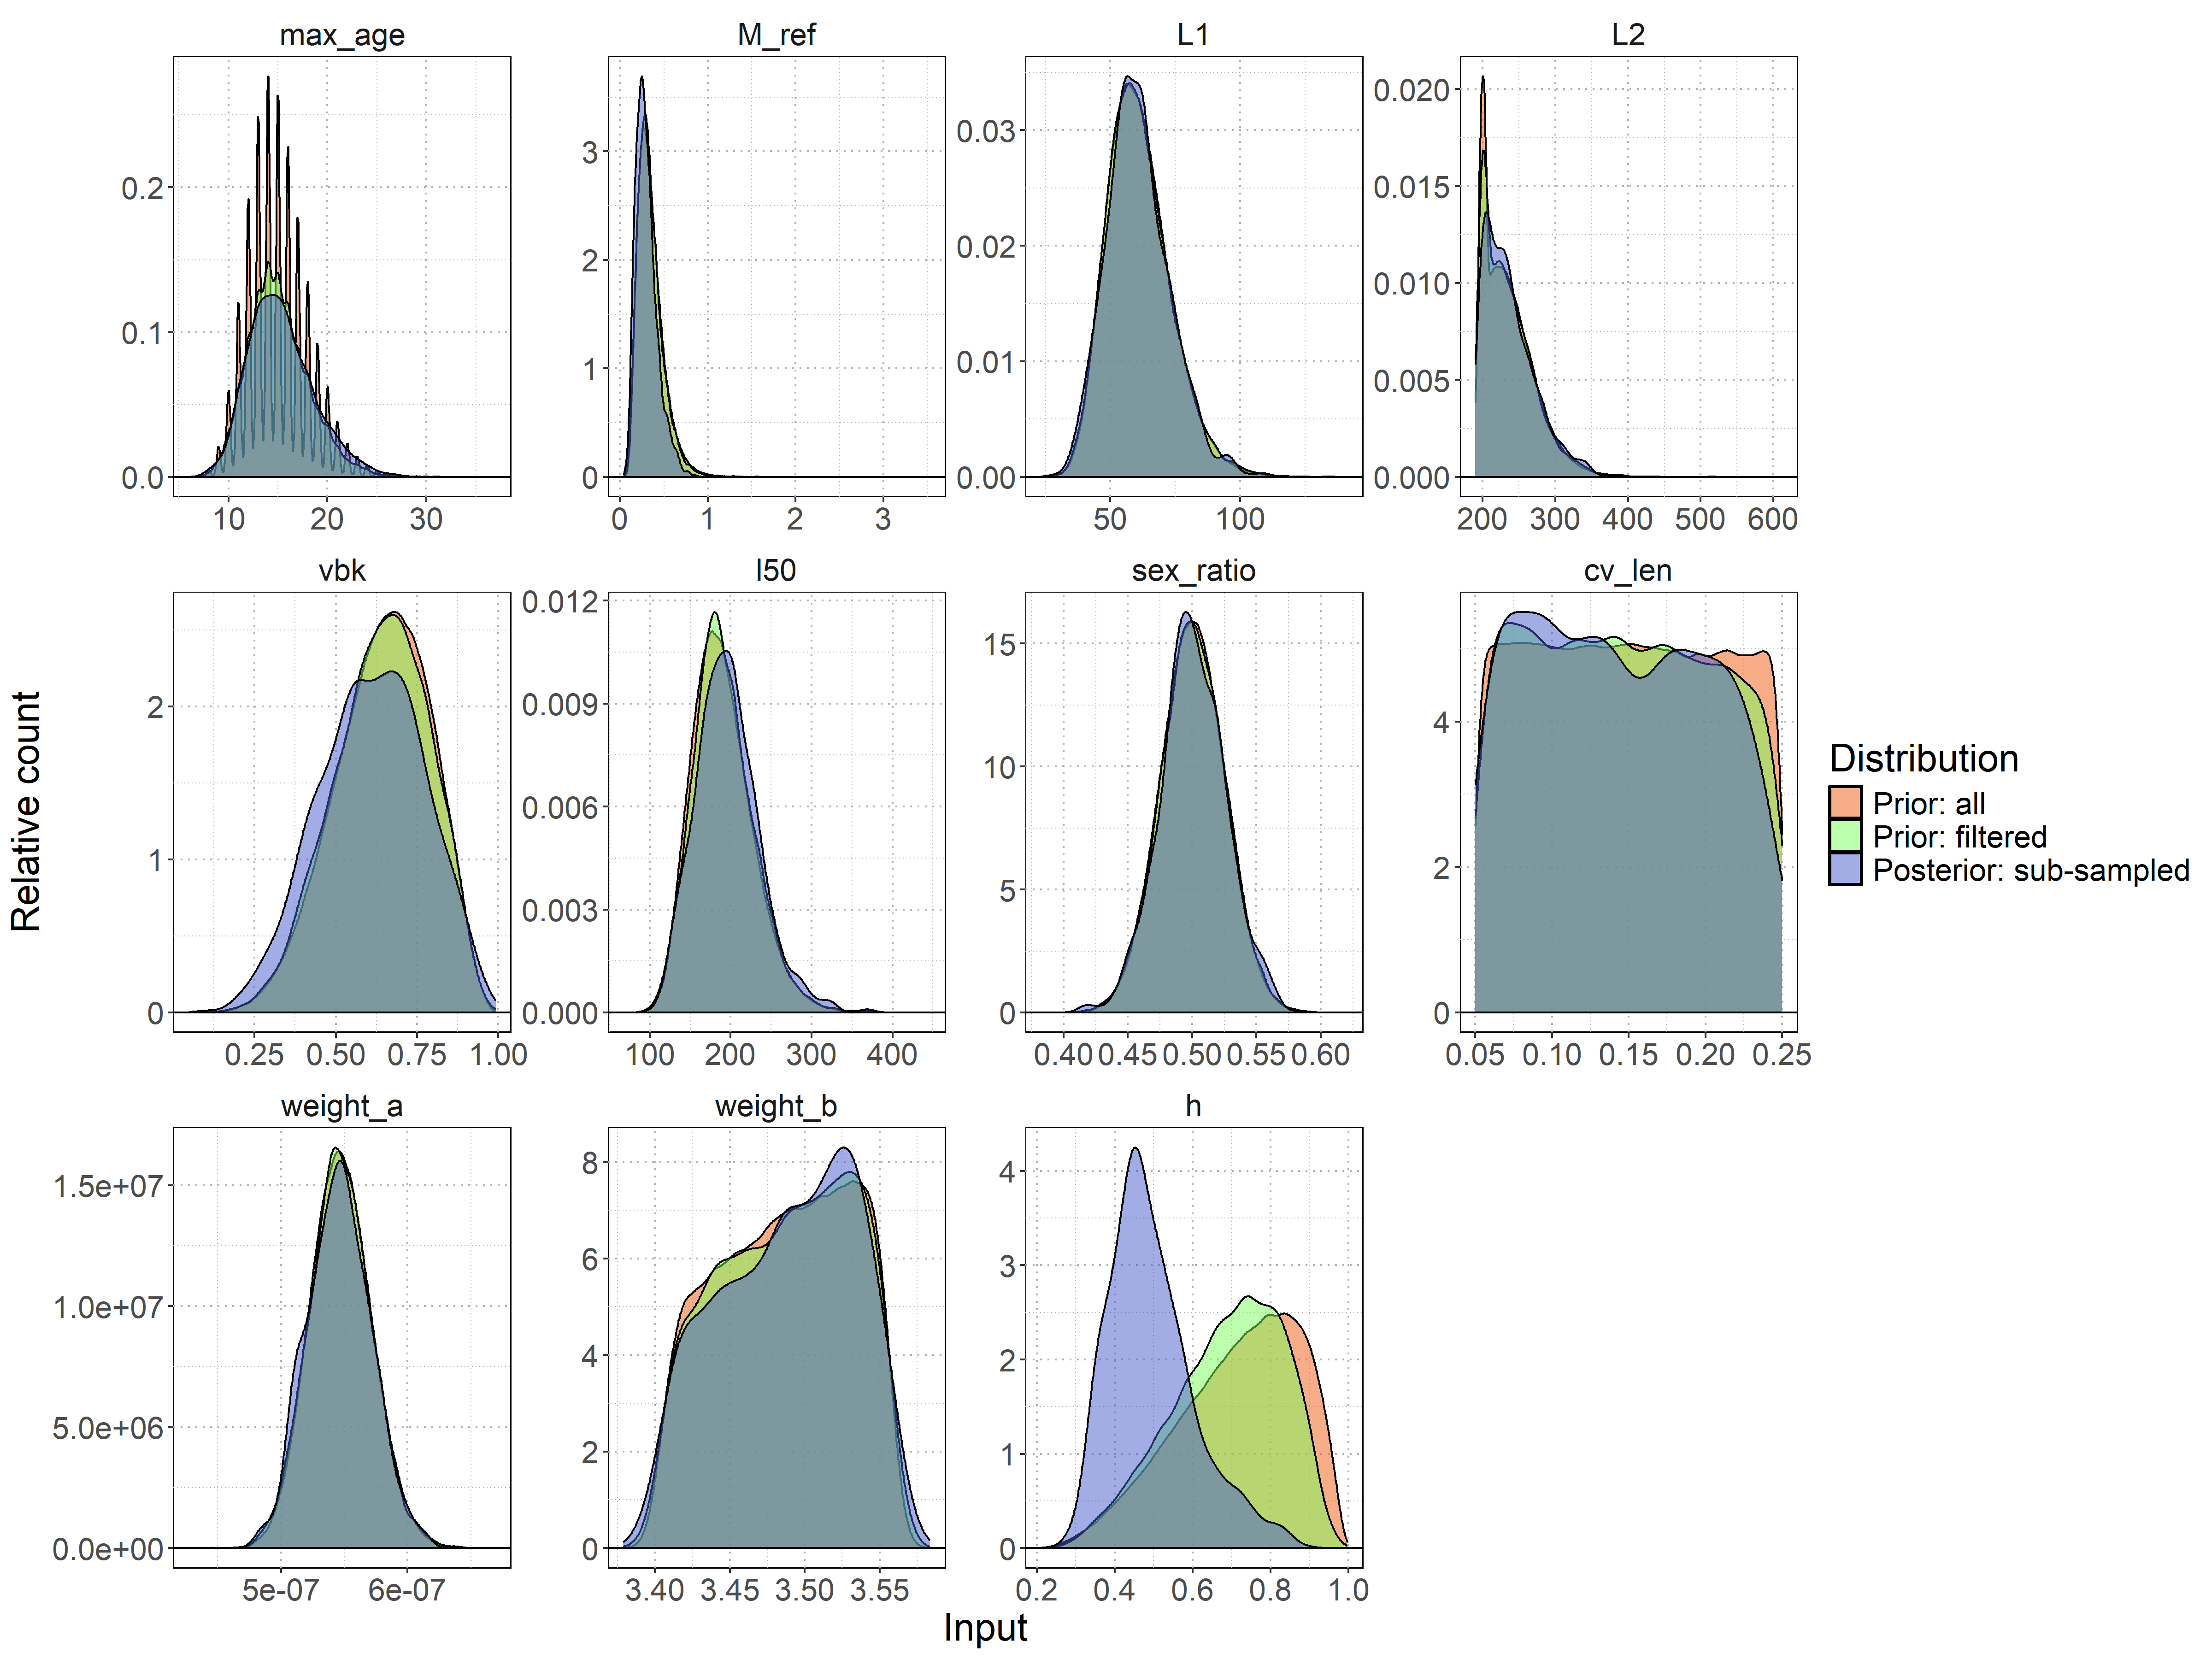
\includegraphics[width=1\linewidth,height=\textheight,keepaspectratio]{../plots/rmax_subsampling_biological_parameters.png}

}

\caption{\label{fig-rmax-subsample-bio}Distributions of biological
parameters (maximum age \emph{max\_age}, natural mortality reference
\emph{M\_ref}, length at birth \emph{L1}, asymptotic length \emph{L2},
von Bertalanffy growth coefficient \emph{vbk}, length at 50\% maturity
\emph{l50}, sex ratio at birth \emph{sex\_ratio}, coefficient of
variation in length \emph{cv\_len}, weight-length relationship
parameters \emph{weight\_a} and \emph{weight\_b}, and steepness
\emph{h}) used in the rmax sub-sampling process. Original biological
prior distribution (orange shading), distribution based on extreme
filtering criteria following the prior pushforward analysis (green
shading), and final sub-sampled distribution selected to match the
posterior \(R_{max}\) distribution (blue shading).}

\end{figure}%

\newpage

\section{Technical Annex}\label{sec-tech-annex}

Additional technical detail of population dynamics components used to
solve the Euler-Lotka equation for \(R_{max}\) and implement the
Gedamke-Hoenig approach (\citeproc{ref-gedamke_estimating_2006}{Gedamke
\& Hoenig, 2006}) for using size composition data to estimate mortality
in non-equilibrium situations.

\subsection{Equilibrium Age-Structured Population
Dynamics}\label{sec-equilibrium-dynamics}

\subsubsection{Survival}\label{sec-survival}

\textbf{Survival schedule} was calculated assuming constant natural
mortality:

\(l_a = \begin{cases}
1 & \text{if } a = 1 \\
l_{a-1} \times \exp(-M_{ref}) & \text{if } 1 < a < A_{max} \\
\frac{l_{A_{max}-1}}{1-\exp(-M_{ref})} & \text{if } a = A_{max} \text{ (plus group)}
\end{cases}\)

\subsubsection{Fecundity}\label{sec-fecundity-calculation}

Reproductive output incorporated biological constraints:
\[f_a = \frac{\psi_a \times W_a \times s}{\rho}\]

where: - \(\psi_a\) = proportion mature at age \(a\) - \(W_a\) = weight
at age \(a\) (proxy for reproductive capacity) - \(s\) = sex ratio
(proportion female) - \(\rho\) = reproductive cycle (years between
spawning events)

\textbf{Maturity-at-age} was derived from length-based logistic
maturity:
\[\psi_L = \frac{\exp(a_{mat} + b_{mat} \times L)}{1 + \exp(a_{mat} + b_{mat} \times L)}\]
where \(b_{mat} = -a_{mat}/L_{50}\), then integrated over the
length-at-age distribution to obtain \(\psi_a\).

\textbf{Length-at-age} followed the Francis parameterization:
\[L_a = L_1 + (L_2 - L_1) \times \frac{1 - \exp(-k(a - age_1))}{1 - \exp(-k(age_2 - age_1))}\]

with length variability modeled using probability density functions
linking length bins to ages.

\textbf{Weight-at-age} used the allometric relationship:
\[W_a = a_w \times L_a^{b_w}\]

\subsubsection{Stock-Recruitment
Relationship}\label{sec-stock-recruitment}

The slope at the origin of the stock-recruitment curve was:
\[\alpha = \frac{4h}{(1-h)\phi_0}\]

The calculation incorporated steepness (\(h\)) through the Beverton-Holt
stock-recruitment relationship. Spawners-per-recruit in the unfished
state was: \[\phi_0 = \sum_{a=1}^{A_{max}} l_a f_a\]

This \(\alpha\) parameter links the intrinsic rate of increase to
recruitment compensation, ensuring that \(R_{max}\) estimates reflect
realistic population productivity under the assumed stock-recruitment
dynamics.

Successful simulations (those yielding \(R_{max} > 0\) and
\(R_{max} < 1.5\)) were filtered to create a plausible prior
distribution (Figure~\ref{fig-pushforward}). The resulting distribution
was fitted to a lognormal prior for use in the BSPM
(Figure~\ref{fig-rmax-prior}).

\subsection{Transitional Mean Weight
Model}\label{sec-transitional-weight-model}

For each biological parameter combination, total mortality rates \(Z_1\)
and \(Z_2\) were estimated by fitting a transitional mean weight model
to observed temporal changes in recreational catch weights. The expected
mean weight during the transition follows:

\[\bar{W}(d) = W_{\infty} - \frac{Z_1 Z_2 (W_{\infty} - W_c) [Z_1 + k + (Z_2 - Z_1)e^{-(Z_2+k)d}]}{(Z_1 + k)(Z_2 + k)[Z_1 + (Z_2 - Z_1)e^{-Z_2 d}]}\]

where: - \(d\) = time since mortality change (years after 1952) -
\(W_{\infty}\) = asymptotic weight from growth parameters - \(W_c\) =
weight at first capture (corresponding to \(L_c\)) - \(k\) = von
Bertalanffy growth coefficient

The mortality parameters were estimated in a likelihood framework by
maximizing the likelihood of the observed mean weights given a time
series of predicted mean weights \(\bar{W}(d)\). Optimization was
constrained such that \(Z_1, Z_2 \geq M_{ref}\) to ensure biologically
realistic mortality estimates.




\end{document}
